\documentclass[a4paper,12pt,oneside]{extbook}
\usepackage{../lectures}
\addbibresource{../finmath.bib}


\title{Финансовая математика --- 2\\[-0.5em]
{\large (<<Модели стохастической волатильности>>)} \\[0.5em]
\Large\it Курс лекций}
\author{Лектор: Михаил Житлухин}

\date{\footnotesize{\texttt{Версия \thedate}}}

\hypersetup{
  pdftitle={Финансовая математика -- 2: Модели стохастической волатильности},
  pdfauthor={Михаил Житлухин}
}

\begin{document}
\onehalfspacing
\maketitle

\tableofcontents
%\addcontentsline{toc}{chapter}{\textbf{О чем этот курс}}
\chapter*{О чем этот курс}

Курс посвящен математической теории \emph{оценивания производных финансовых инструментов} таких как опционы, фьючерсы и \tp\ 
Основная его цель "--- познакомить с фундаментальными идеями, используемыми в этой области, и изучить их на примере базовых моделей.
Этот курс в разное время читался и продолжает читаться в Высшей школе экономики на факультетах МИЭФ и ФКН, а также в МГУ на механико-математическом факультете и в рамках программы Института <<Вега>>. 

В первой части курса будут рассмотрены модели с дискретным временем, в во второй части "--- модели с непрерывным временем.
При изучении моделей с непрерывным временем мы также обсудим основы стохастического исчисления, которые нам потребуются: интеграл Ито, формула Ито, стохастические дифференциальные уравнения и \tp\ 
Эти понятия интересны и важны сами по себе.
Курс завершается на модели \bs\ и ее вариантах.

Стоит отметить, что модели, изучаемые в этом курсе, слишком просты, чтобы применять их на практике, однако они задают фундамент для продвинутой теории, которая излагается в курсах <<Модели стохастической волатильности>> (<<Финансовая математика --- 2>>) и <<Финансовая математика --- 3>>\footnote{Курс <<Финансовая математика --- 3>> пока не читается, но когда-нибудь будет.}.

Курс рассчитан на один семестр. Часть материала оставлена для самостоятельного изучения и не входит в экзамен; она вынесена в раздел <<Дополнения>>.
Также по ходу изложения некоторые разделы отмечены звездочками "--- это дополнительный материал, который более труден, чем средний уровень курса.

%Раздел <<Практикум>> посвящен решению задач по финансовой математике на языке Python и может служить первой частью самостоятельного курса по программированию финансовых моделей.

Для полного освоения курса желательно иметь уверенное знания теории вероятностей и наличие  базовых представлений о финансовых рынках.
%Для освоения практической части требуется умение программировать на языке Python.

%!TEX root=finmath2.tex
\chapter{Почему волатильность стохастическая?}
\chaptertoc

В этой лекции мы перечислим эмпирические факты, показывающие, что модель \bs\ не может адекватно описывать рыночные цены, и обсудим почему возникает необходимость в более продвинутых моделях, в которых волатильность задается случайным процессом.

\section{Напоминание: модель \bs}
В модели \bs\ цены безрискового и рискового активов задаются уравнениями
\[
d B_t = rB_t dt, \qquad
d S_t = \mu S_t dt + \sigma S_t d W_t.
\]
Для простоты будем считать, что рисковый актив не платит дивиденды, а безрисковая процентная ставка постоянна.
Решение уравнения для $S_t$ (геометрическое броуновское движение) представляется в виде
\[
S_t = S_0 e^{\sigma W_t + (\mu-\frac{\sigma^2}{2})t}.
\]

Для вычисления цен производных инструментов (платежных обязательств) нужно перейти к эквивалентной мартингальной мере $\Q$, относительно которой
\[
d S_t = r S_t dt + \sigma S_t d W_t^{\Q},
\]
где $W^{\Q}$ "--- броуновское движение относительно $\Q$.
Тогда цена европейского платежного обязательства в момент времени 0 с выплатой $X$, производимой  в момент $T$, вычисляется по формуле
\[
V = e^{-rT} \E^Q X.
\]
Для европейских опционов колл и пут математическое ожидание можно вычислить явно, что дает формулу \bs\ (см.~курс <<Введение в финансовую математику>>).
% \[
% \VC = S_0 \Phi(d_1) - K e^{-rT} \Phi(d_2), \qquad
% \VP = K e^{-rT} \Phi(-d_2) - S_0 \Phi(-d_1),
% \]
% где $\Phi(x)$ обозначает стандартную нормальную функцию распределения и
% \[
% d_1 = \frac{\ln(S_0/K) + (r+\sigma^2/2)T}{\sigma\sqrt T}, \qquad 
% d_2 = d_1 - \sigma\sqrt T.
% \]


\section{Почему модель \bs\ не согласуется с рыночными данными}
\subsection{Свойства вероятностных распределений рыночных цен}
\subsubsection{Отсутствие нормальности}

Для временного ряда рыночных цен с шагом $\Delta t$, \te\ $S_0, S_{\Delta t}, S_{2\Delta t},\dots$, построим последовательность
\[
L_t = \ln S_t - \ln S_{t-\Delta t}, \qquad t\in \{\Delta t, 2\Delta t,\dots\}.
\]
Если бы цены следовали модели \bs, то последовательность $L_t$ представляла бы реализацию последовательности независимых и одинаково распределенных нормальных случайных величин со средним $(\mu-\sigma^2/2)\Delta t$ и дисперсией $\sigma^2\Delta t$.

Из примера на рис.~\ref{intro:f:real-vol} видно, что это не так.
Левый график на этом рисунке изображает последовательность $L_t$ для индекса SnP~500 за 2015--2024 гг.\ с $\Delta t$ равным 1 дню, а правый график "--- симулированную последовательность нормальных величин с такими же средним и дисперсией. 
Характер графиков качественно отличается, что говорит о том, что распределение приращений значения индекса не является нормальным.
Аналогичная картина наблюдается и для других активов.

Ненормальность распределения подтверждается и гистограммой на рис.~\ref{intro:f:hist}.
Если бы данные были нормальными, то гистограмма была бы близка к графику плотности нормального распределения, но видно, что их формы отличаются.


\subsubsection{Ассимметрия и тяжелые хвосты}

Различие между эмпирическим распределением $L_t$ и нормальным распределением можно также увидеть из простых численных характеристик.
Например, вычислим выборочные коэффициенты асимметрии и эксцесса
\[
\gamma = \frac{\mu_3}{\sigma^3}, \qquad \kappa = \frac{\mu_4}{\sigma^4} - 3,
\] 
где $\mu_3,\mu_4$ "--- выборочные 3-й и 4-й центральные моменты, а $\sigma$ "--- выборочное стандартное отклонение.
Для выборки, полученной из нормального распределения, $\gamma$ и $\kappa$ будут близки к нулю (соответствующие теоретические коэффициенты для нормального распределения в точности равны 0), но в рассматриваемом примере с индексом SnP 500 получаются значения $-0.81$ и $15.7$.

Отрицательность коэффициента асимметрии говорит о том, что распределение скошено влево, а положительность коэффициента эксцесса "--- о том, что распределение имеет более <<тяжелые>> хвосты по сравнению с нормальным распределением.

\begin{figure}[t]
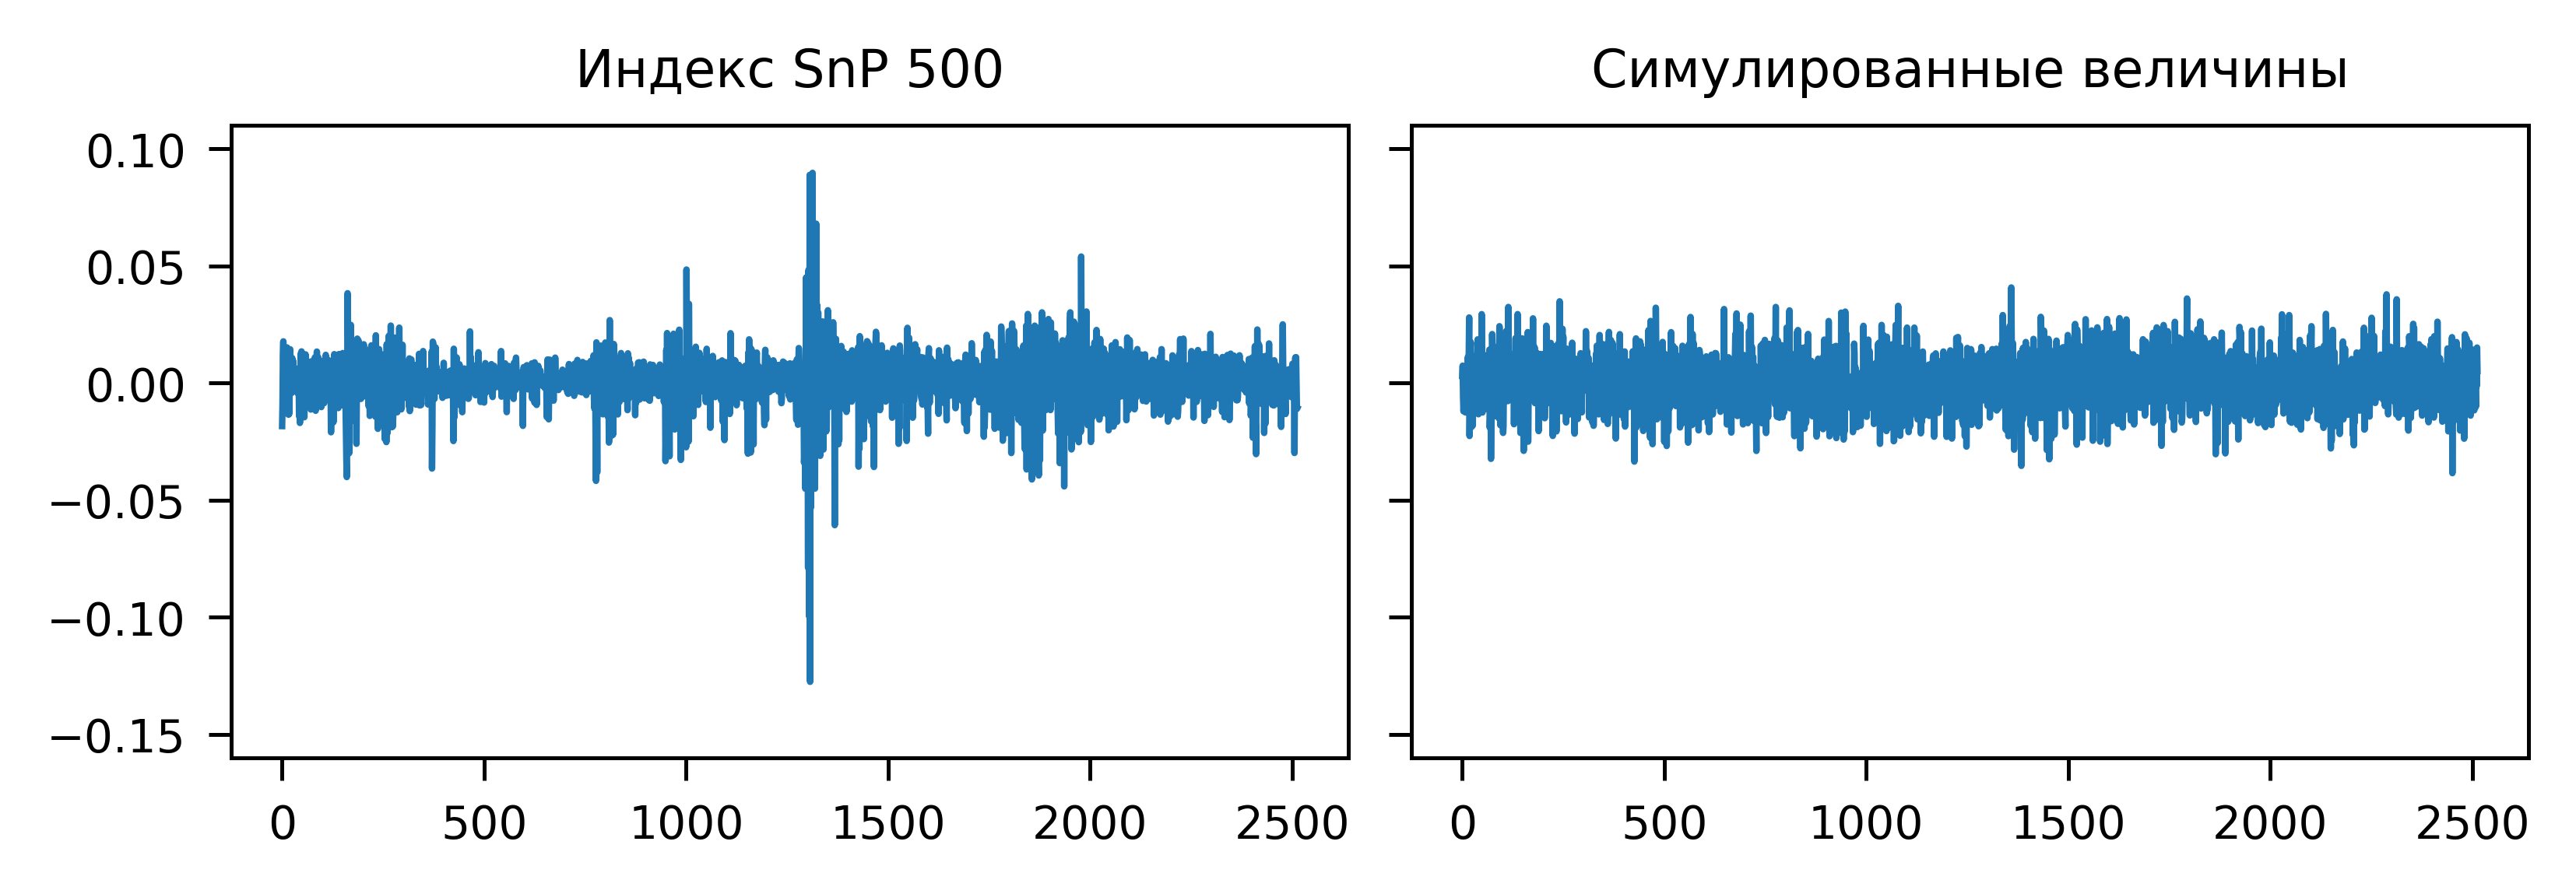
\includegraphics{pic/snp-returns.png}
\centering
\caption{Приращения логарифмов значений индекса SnP 500 и симулированные нормальные случайные величины с такими же средним и дисперсией.}
\label{intro:f:real-vol}
\end{figure}

\begin{figure}[t]
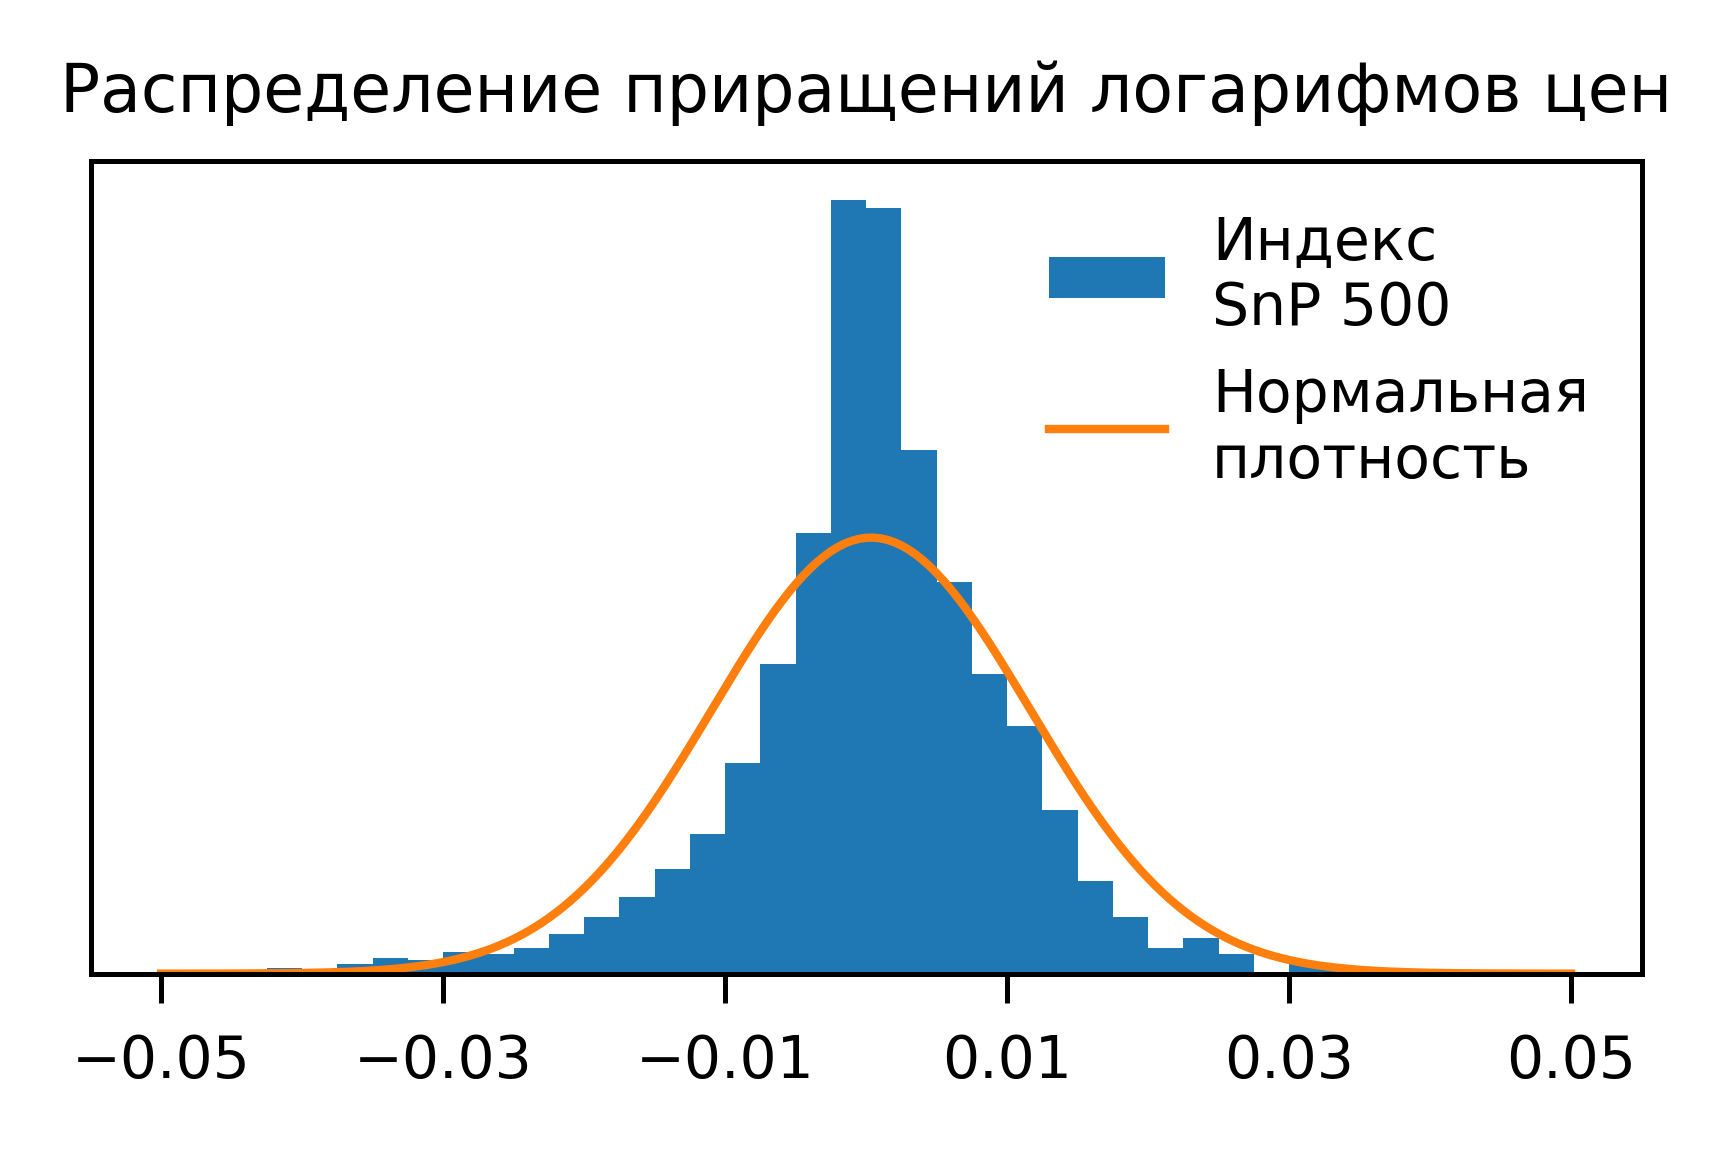
\includegraphics{pic/snp-hist.png}
\centering
\caption{Сравнение эмпирического распределения приращений логарифмов индекса SnP 500 с нормальным распределением.}
\label{intro:f:hist}
\end{figure}


\subsubsection{Автокорреляция}

Для геометрического броуновского движения величины $L_{t+s}$ и $L_t$ независимыми при $s\ge \Delta t$ в силу независимости приращений броуновского движения.
Из независимости следует некоррелированность, поэтому можно вычислить эмпирические коэффициенты корреляции (\te\ автокорреляционную функцию) и посмотреть, близки ли они к нулю.
Оказывается, что для рыночных данных корреляции $\rho(L_{t+s},L_t)$ близки к нулю, но корреляции квадратов приращений логарифмов $\rho(L_{t+s}^2,L_t^2)$ отличается от нуля (см.~рис.~\ref{intro:f:autocorr}).
Это говорит о том, что величины $L_{t+s}$ и $L_t$ зависимы, хотя и слабо коррелированны. 

\begin{figure}[t]
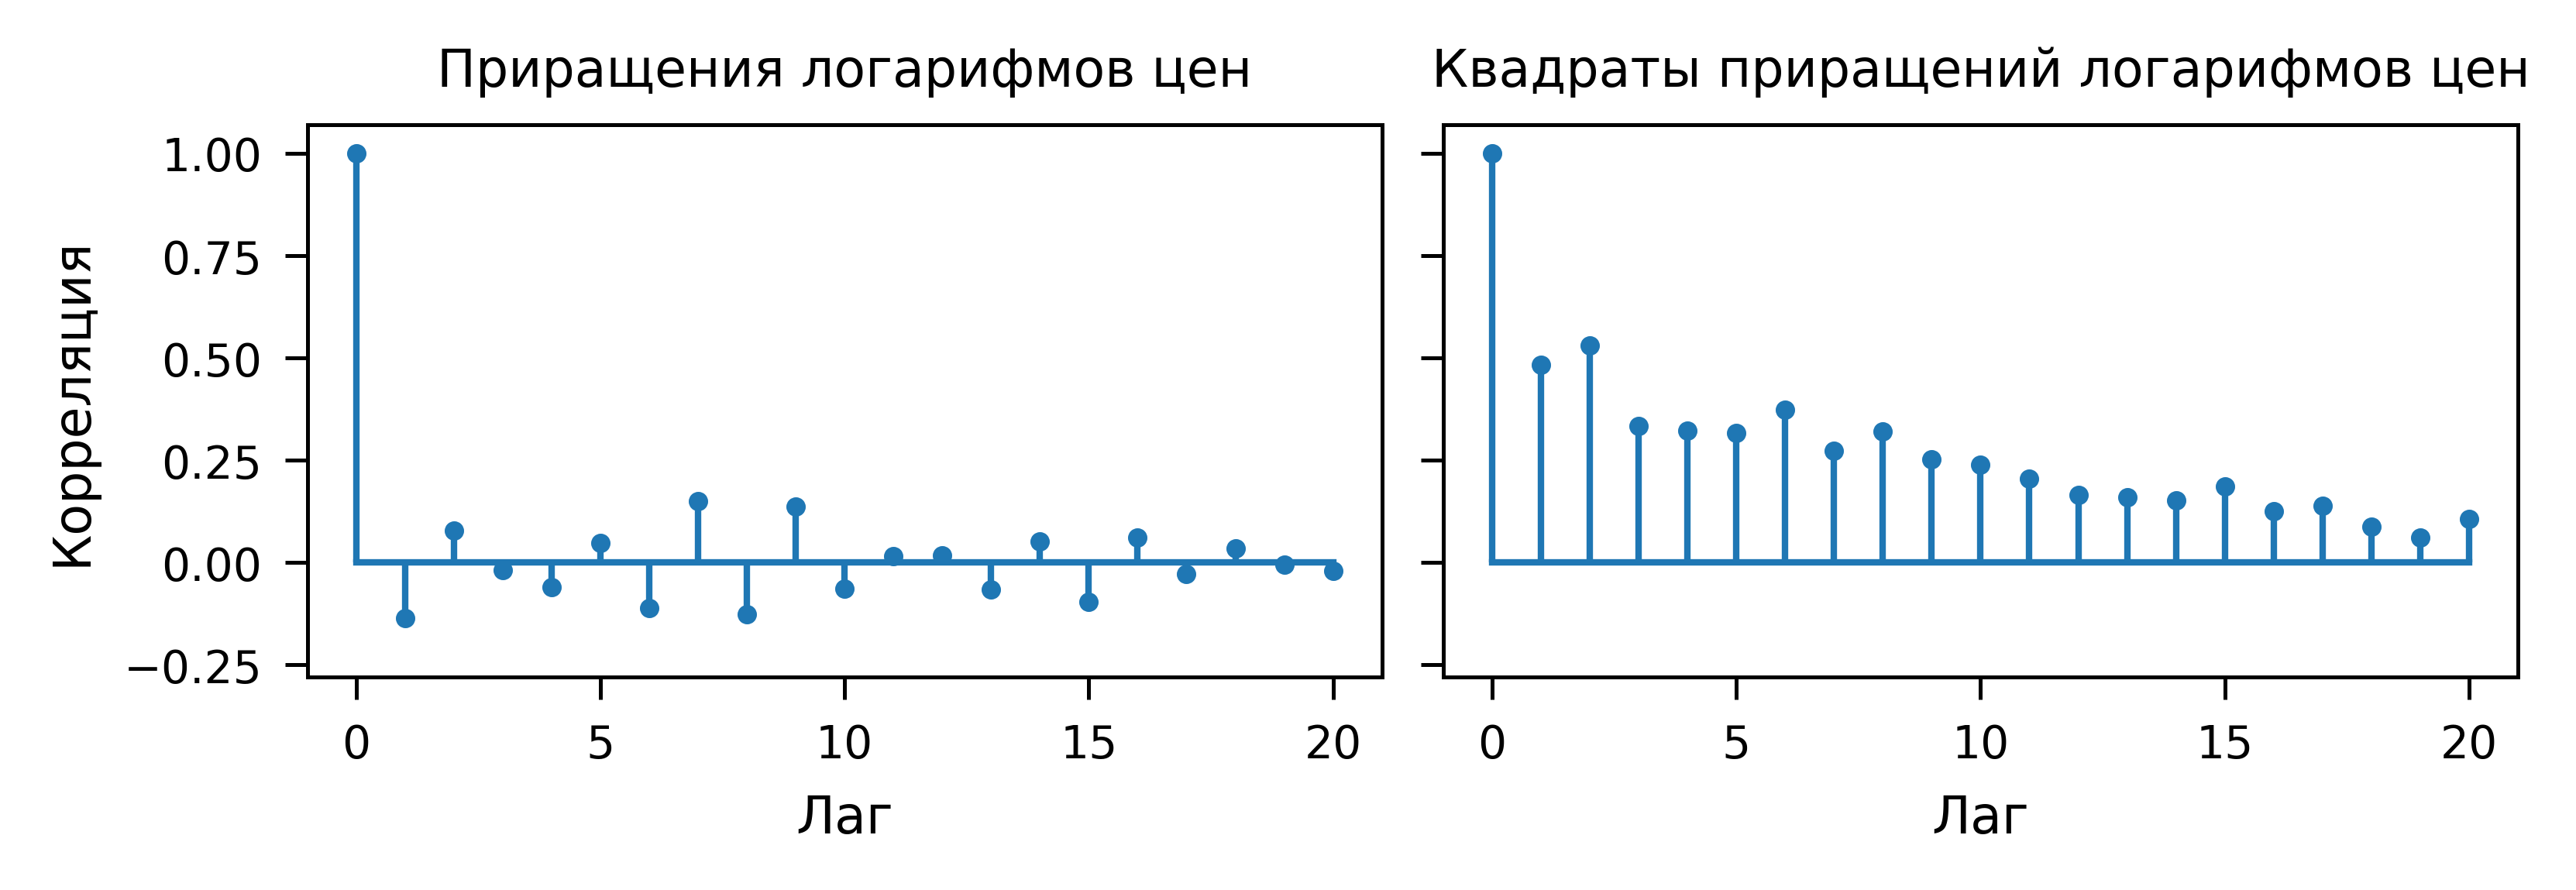
\includegraphics{pic/snp-autocorr.png}
\centering
\caption{Автокорреляционная функция для логарифмов приращений значения индекса SnP 500 и квадратов логарифмов приращений.}
\label{intro:f:autocorr}
\end{figure}


\subsubsection{Другие эмпирические факты}

Обзор статистических свойств рыночных цен приведен в статье \cite{Cont01}.
Эти свойства также называются \emph{стилизованными фактами}.
Кратко перечислим некоторые стилизованные факты, отсылая за подробностями к упомянутой статье.
\begin{itemize}
\item Имеется зависимость между изменениями цены и изменениями волатильности: часто при падении цены волатильность возрастает, а при росте цены остается без существенных изменений или плавно уменьшается. В модели \bs\ такого быть не может, так как величина $\sigma$ постоянна.

\item Кластеризация волатильности: за большими значениями волатильности преимущественно следуют большие значения, за малыми "--- малые.
Если представлять волатильность как степень <<беспокойства>> рынка, то это означает, что на рынке наблюдаются периоды спокойствия и беспокойства.
В модели \bs, напротив, рынок всегда <<одинаково спокоен>>.

\item Присутствие <<скачков>> (\te\ разрывов) в процессах цен, которые нельзя объяснить только тем, что данные собираются дискретным образом.%
\footnote{В этом курсе мы будем рассматривать модели, в которых процессы цен непрерывны.
Модели со скачками, основанные на \emph{процессах Леви}, были популярны в 2000-x гг.}
\end{itemize}


\subsection{Подразумеваемая волатильность}

На ликвидных рынках цены опционов можно считать известными (из рыночных данных), и тогда для каждого опциона можно найти значение $\sigma$ такое, что цена, вычисленная по формуле \bs, совпадает с рыночной ценой "--- это значение $\sigma$ называется \emph{подразумеваемой волатильностью}.
Мы будем обозначать его как $\hat\sigma(T,K)$, когда нужно подчеркнуть зависимость от страйка и времени исполнения.

Если бы рыночные данные следователи модели \bs, то построенная по ним функция $\hat\sigma(T,K)$ была бы постоянной и равнялась параметру волатильности в модели.
В реальности это не так.
Например, на рис.~\ref{intro:f:smiles} приведены \emph{улыбки волатильности}%
\footnote{Улыбкой волатильности называется функция $\hat\sigma(T,K)$, рассматриваемая как функция от страйка $K$ с фиксированным значением $T$.}
для опционов на индекс S\&P 500 с разными датами исполнения.
Видно, что функция $\hat\sigma(T,K)$ не постоянна как по $K$, так и по $T$.

Это приводит к трудности выбора параметра волатильности в модели \bs\ для оценки экзотических производных инструментов.
Например, следует ли для оценки барьерного опциона взять подразумеваемую волатильность, соответствующую страйку, равному барьеру, или страйку, равному текущей цене базового актива?
Хотелось бы иметь модель, которая позволяет оценивать деривативы, без изменения ее параметров под каждый инструмент.

\begin{figure}[t]
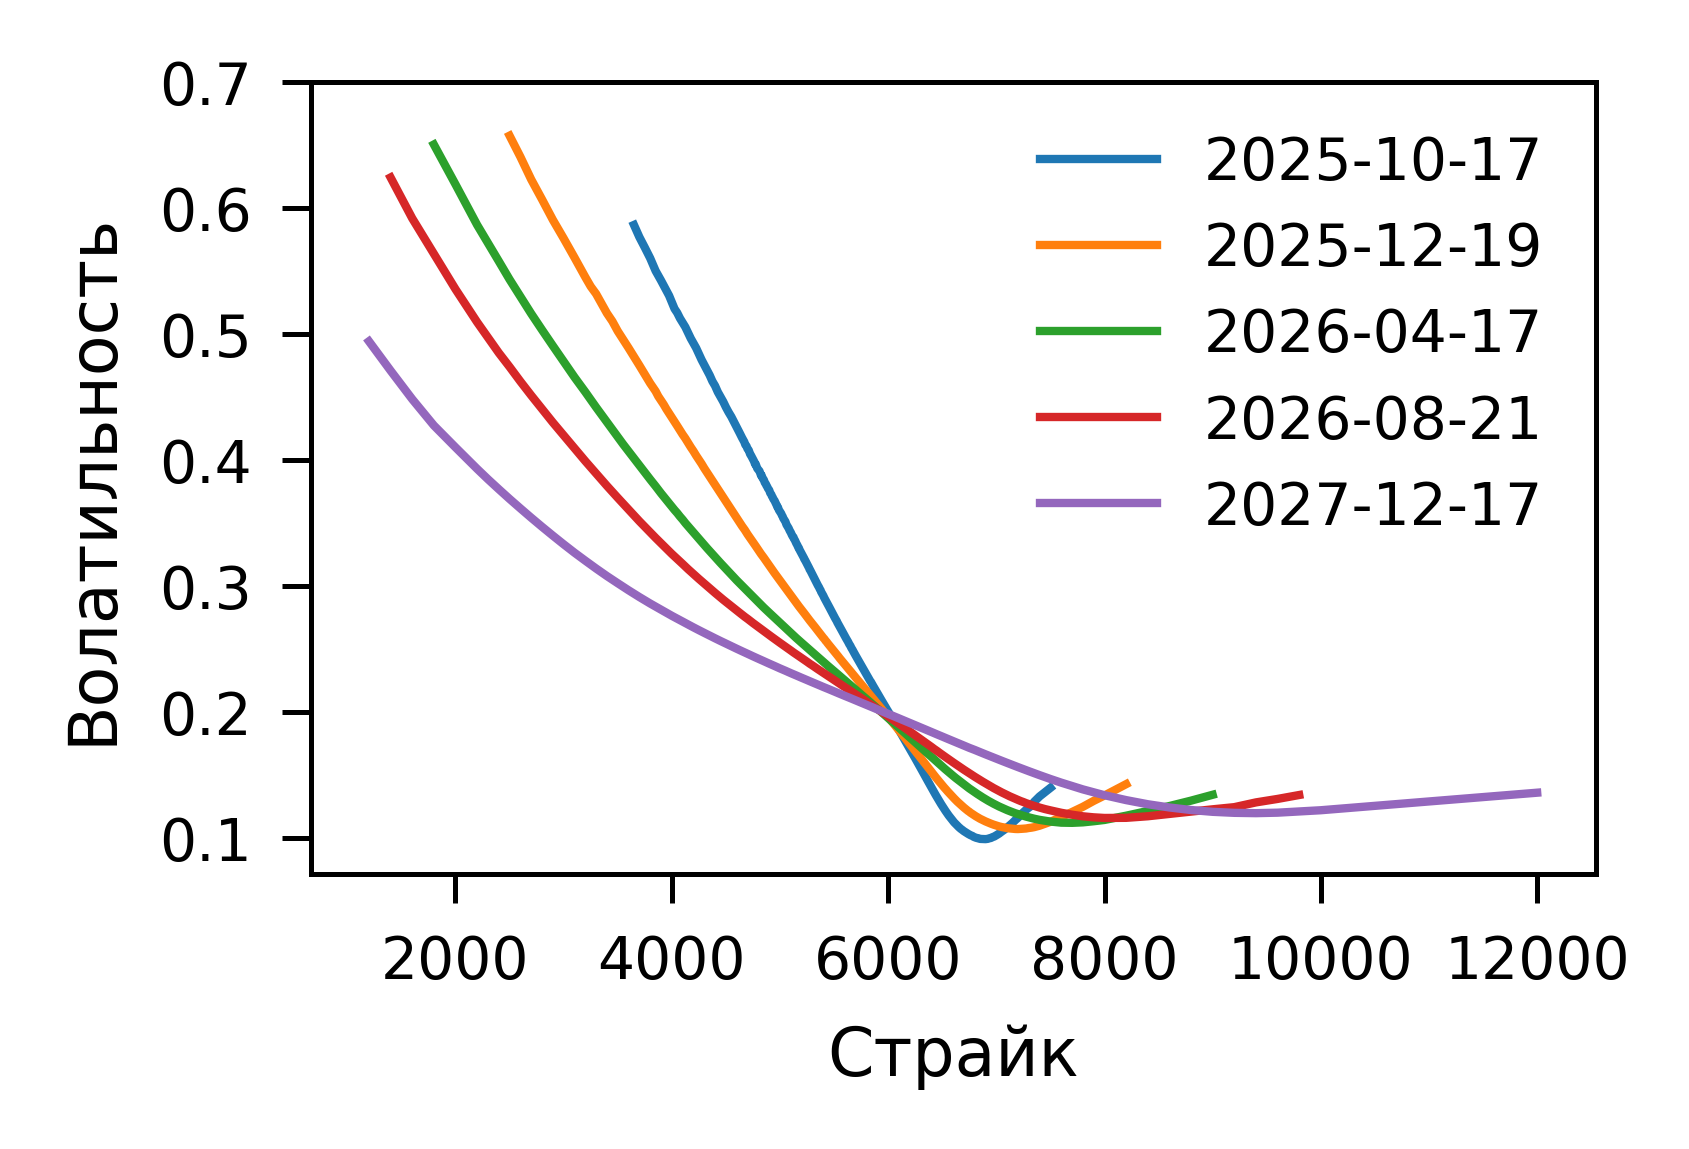
\includegraphics[height=5cm]{pic/snp-smiles.png}
\centering
\caption{Улыбки волатильности для индекса SnP 500 с разными датами исполнения, построенные по ценам опционов на дату  25.04.2024.}
\label{intro:f:smiles}
\end{figure}


\subsection{К каким ошибкам приводит модель \bs?}

Рассмотрим два типа ошибок, свойственных всем моделям и, в том числе, модели \bs.
Естественно, чем ошибка в модели меньше, тем модель лучше.
Соответственно, целью исследования более сложных моделей цен является, в том числе, нахождение моделей дающих меньшие ошибки.

\subsubsection{Статическая ошибка}
Под \emph{статической ошибкой} модели мы будем понимать несоответствие между рыночными ценами ликвидных (т.е.\ активно торгующихся и имеющих доступные рыночные цены) производных инструментов%
\footnote{Под ликвидными производными инструментами далее, в основном, имеются ввиду ванильные европейские опционы колл и пут.}
и ценами этих инструментов, получаемых в модели.

Статическая ошибка приводит к следующему нежелательному эффекту: модель дает цены инструментов, по которым их невозможно купить или продать.
Отметим, что статическая ошибка означает не то, что параметры модели неправильно откалиброваны к рыночным данным, а то, что модель в принципе не способна попасть в набор цен деривативов ни при каких комбинациях своих параметров.

В модели \bs\ статическая ошибка возникает из-за того, что в ней предполагается постоянство волатильности:
каким бы ни был параметр $\sigma$, модель не может воспроизвести рыночные улыбки волатильности, что означает невозможность воспроизвести рыночные цены ванильных опционов.


\subsubsection{Динамическая ошибка}

Под \emph{динамической ошибкой} мы будем понимать несоответствие между вероятностными распределениями процессов цен базовых активов, процессов цен ликвидных производных инструментов, а также других динамических характеристик%
\footnote{Например, такими характеристиками могут быть величины, вычисляемые из поверхности волатильности: волатильность опционов ATM, наклон и кривизна поверхности, и др.}, которые получаются в модели и наблюдаются в реальных данных. 

Динамическая ошибка приводит к ошибке репликации: производные инструменты, которые в выбранной модели теоретически можно реплицировать с помощью самофинансируемых стратегий, не реплицируются в точности.

Поясним на примере.
Пусть требуется реплицировать платежное обязательство, производящее выплату $X$ в момент времени $T$.
Для простоты предположим, что процентная ставка равна нулю, а $X$ зависит только от $S_T$, \te\ $X=f(S_T)$.
Если использовать для репликации модель \bs, то количество рискового актива $H_t$ в реплицируемом портфеле $\pi_t$ должно быть равно дельте инструмента:
\[
H_t = V'_s(t,S_t),
\]
где $V_t(t,s) = \E^{\Q} (f(S_T) \mid S_t=s)$ "--- его цена в модели \bs.
Тогда стоимость портфеля $\pi_t$ в момент исполнения будет равна
\[
V_T^\pi = V(0,S_0) + \int_0^T H_t d S_t = V(0,S_0) + \int_0^T V'_s(t,S_t) d S_t.
\]
С другой стороны, по формуле Ито имеем
\[
V(T,S_T) = V(0,S_0) + \int_0^T V'_t(t,S_t) dt + \int_0^T V'_s(t,S_t) d S_t + \frac12 \int_0^t V''_{ss}(t,S_t) (dS_t)^2.
\]
Так как $X=V(T,S_T)$, то для \emph{ошибки репликации} $\epsilon := V_T^\pi - X$ получаем выражение
\[
\epsilon = \int_0^T V'_t(t,S_t) dt + \frac12 \int_0^t V''_{ss}(t,S_t) (dS_t)^2.
\]

Далее воспользуемся тем, что $V'_t(t,s) = -\frac12 \sigma^2 V''_{ss}(t,s)$, как следует из уравнения \bs\ (при нулевой безрисковой ставке); здесь $\sigma$ "--- параметр волатильности в модели, используемой для репликации.
Если же допустить, что в реальности процесс цены $S_t$ имеет стохастическую волатильность, \te\ $dS_t = \sigma_t S_t d W_t$ со случайным процессом $\sigma_t$, то получим ненулевую ошибку:
\[
\epsilon = \frac12 \int_0^T (\sigma_t^2 - \sigma^2) V''_{ss}(t,S_t)S_t^2 dt.
\]

%%%%%%%%%%%%%%%%%%%%
% Старый фрагмент, непонятно написан
%%%%%%%%%%%%%%%%%%%%
% Рассмотрим функцию $V(t,S_t)$ такую, что $V(T,s) = g(s)$ (пусть пока $V$ произвольна, потом будет видно, как она связана с ценой платежного обязательства).
% Тогда портфель, состоящих из безрискового и рискового актива, стоимость которого в каждый момент времени равна $V(t,S_t)$, реплицирует $X$.
% Будем считать, что портфель не обязательно является самофинансируемым, и величина притока/оттока капитала описывается дифференциалом $C_t dt$.
% Тогда необходимо, чтобы было выполнено равенство $d V(t,S_t) = h_tdS_t + C_t dt$, где $h_t$ "--- количество единиц рискового актива в портфеле. По формуле Ито это эквивалентно равенству
% \[
% C_t dt = V'_t(t,S_t) dt + V'_s(t,S_t) dS_t + \frac12 V''_{ss}(t,S_t) (dS_t)^2 - h_t d S_t.
% \]
% Если выбрать $h_t=V'_s(t,S_t)$, то слагаемые с $dS_t$ сократятся, что уберет зависимость от изменения цены базового актива с точностью до первого порядка (<<дельта-хеджирование>>).
% Подставляя $(dS_t)^2 = \sigma^2 S_t^2 dt$, получаем
% \[
% C_t dt = \left(V'_t(t,S_t) + \frac{\sigma^2}2 V''_{ss}(t,S_t)S_t^2\right) dt.
% \]
% В модели \bs\ величина $\sigma$ постоянна.
% Поэтому, если предполагать, что модель верна, то можно найти функцию $V$ из уравнения в частных производных 
% \begin{equation}
% \label{intro:v}  
% V'_t + \frac{\sigma^2}{2} V''_{ss} = 0
% \end{equation}
% с терминальным условием $V(T,s) = f(s)$, что даст нулевой приток капитала $C_t$, и, таким образом, получится самофинансируемый портфель, который реплицирует $X$.

% Если же допустить, что волатильность $\sigma$ не постоянна, то получим (по-прежнему считая, что $V$ удовлетворяет \eqref{intro:v})
% \[
% C_t = \frac{\sigma_t^2-\hat\sigma^2}{2} V''_{ss}(t,S_t) S_t^2, 
% \]
% где $\hat\sigma$ "--- значение волатильности, которое использовалось при решении уравнения \eqref{intro:v}.
% Таким образом, денежная величина ошибки хеджирования составит
% \[
% C_T = \int_0^T \frac{\sigma_t^2-\hat\sigma^2}{2} V''_{ss}(t,S_t) S_t^2 dt.
% \]
% Тот факт, что $C_T$ не равно нулю означает наличие ошибки репликации.
% Она здесь возникла из-за того, что в модели предполагается постоянство коэффициента $\sigma$, а в реальности $\sigma_t$ не постоянно.
%%%%%%%%%%%%%%%%%%%%

\section{Краткая история моделей стохастической волатильности}

Под моделями стохастической волатильности мы будем понимать модели, в которых процесс цены базового актива относительно эквивалентной мартингальной меры имеет вид
\[
dS_t = r_tS_t dt + \sigma_t S_t dW_t,
\]
где $r_t$ "--- безрисковая процентная ставка (в этом курсе она будет, как правило, считаться детерминированной функцией), a $\sigma_t$ "--- случайный процесс\footnote{В случае, когда $\sigma_t$ является функцией только от текущего значения цены $S_t$ и времени, волатильность часто называют \emph{локальной}, а не стохастической; см.~далее.}.
Замена постоянного параметра $\sigma$ в модели \bs\ на случайный процесс приводит к большому разнообразию получаемых моделей. 

Далее перечислим некоторые известные модели стохастической волатильности, кратко упомянув их достоинства и недостатки.
При первом чтении этого раздела многое может показаться непонятным.
К нему стоит вернуться после окончания курса.

\subsubsection{Модель CEV}

Первой моделью стохастической волатильности была \emph{модель CEV}\footnote{Constant Elasticity of Variance "--- модель c постоянной эластичностью дисперсии.}, предложенная Дж.~Коксом (J.~Cox, 1975).
Уравнение цены в ней имеет вид
\[
d S_t = r_tS_t dt + \sigma S_t^\gamma d W_t,
\]
где $\gamma \ge 0$ и $\sigma>0$ "--- параметры модели. Таким образом, здесь $\sigma_t = \sigma S_t^{\gamma-1}$. 
При $\gamma=1$ получается модель \bs, а при $\gamma=0$ "--- модель Башелье.

Если $\gamma\in[0,1)$, то волатильность растет, когда цена падает, и падает, когда, цена растет.
В первом приближении такое поведение действительно наблюдается в ценах акций.
Кроме того, улыбки волатильности в модели CEV при $\gamma\in(0,1)$ получаются скошенными вправо, что тоже в некоторой степени соответствует наблюдаемым данным.
Если $\gamma>1$, то получается противоположное поведение, которое не характерно для рынков акций, но, может наблюдаться, например, на рынках товаров.

У модели CEV имеется два недостатка.
Во-первых, она недостаточно гибкая, чтобы правильно описывать наблюдаемые поверхности подразумеваемой волатильности (у нее всего два параметра).

Во-вторых, функциональная зависимость $\sigma_t=\sigma(S_t)$ означает, что волатильность зависит только от текущего уровня цены, но в реальности на изменение волатильности оказывают влияние и другие факторы.
Можно провести такой мысленный эксперимент.
Пусть сегодня акция стоит 100, а через год будет стоить 120.
Если за этот год цена акции будет расти <<равномерно>> то можно ожидать, что к концу года волатильность будет в пределах своих <<обычных>> значений.
Однако, если за первые 11 месяцев цена вырастет до 180, а за последний месяц упадет до 120, то волатильность будет высокой. 
В модели CEV, напротив, в обоих случаях волатильность должна быть одинаковой.


\subsubsection{Модель локальной волатильности}

Модель локальной волатильности, предложенная Б.~Дюпиром (B.~Dupire, 1994), решает проблему статической ошибки: она в точности калибруется к ценам наблюдаемых европейских опционов.
Модель имеет вид
\[
d S_t = r_tS_t dt + \sigma(t,S_t) d W_t,
\]
где $\sigma(t,s)$ "--- детерминированная функция, которая определяется из рыночных цен опционов по некоторой аналитической формуле.

Несмотря на отсутствие статической ошибки, в модели локальной волатильности присутствует динамическая ошибка по той же причине, что и в модели CEV "--- из-за жесткой связи волатильности и цены.


\subsubsection{Модель Хестона}
Одной из наиболее известных моделей стохастической волатильности является модель C.~Хестона (S.~Heston, 1993).
Она задается уравнениями
\begin{align*}
&d S_t = r_tS_tdt + \sqrt{V_t} d W_t^{(1)},\\
&d V_t = \kappa(\theta - V_t)dt + \sigma \sqrt{V_t} d W_t^{(2)},\\
&d W_t^{(1)} d W_t^{(2)} = \rho dt,
\end{align*}
где процесс $V_t$ называется стохастической дисперсией (а $\sigma_t = \sqrt{V_t}$ "--- стохастической волатильностью).
Величины $\kappa,\theta,\sigma,\rho, V_0$ "--- параметры модели.
Третье уравнение означает, что броуновские движения $W_t^{(1)}$ и $W_t^{(2)}$ являются коррелированными с коэффициентом корреляции $\rho$ (\te\ $\E W_t^{(1)}W_t^{(2)} = \rho t$).

Пять параметров придают модели Хестона достаточно гибкости в подгонке к рыночным ценам опционов, но она все равно имеет статическую ошибку "--- это неизбежно при конечном числе параметров.
С другой стороны, зависимость волатильности от дополнительного случайного фактора позволяет более правильно отражать ее динамику по сравнению с моделью локальной волатильности. 

Большим достоинством модели Хестона является наличие эффективного способа вычисления цен европейских опционов, что необходимо для калибровки параметров модели.
Это важное свойство любой модели "--- можно придумать много разных уравнений, задающих стохастическую волатильность, но если нет эффективного метода вычисления цен простых деривативов, то такую модель модель будет трудно использовать на практике.

%%%%%%%%%%%%%%%%%%%%
%%% Непонятный абзац
%%%%%%%%%%%%%%%%%%%%
% Из недостатков модели Хестона можно отметить то, что она является недостаточно гибкой для описания динамики поверхности подразумеваемой волатильности.
% А именно, если откалибровать параметры модели по наблюдаемой поверхности подразумеваемой волатильности в текущий момент времени, то эти параметры будут также определять вероятностное распределение того, как вся поверхность будет двигаться в последующие моменты времени: грубо говоря, получается, что начальное значение процесса жестко связано с его распределением.
% Хотелось бы иметь параметры, которые будут отдельно контролировать динамику волатильности.
% Это необходимо для оценки экзотических деривативов, которые зависят от будущих значений волатильности (например, опционов с форвардным стартом). 

В дополнение к модели Хестона упомянем некоторые другие модели, в которых волатильность задается диффузионным процессом; эти модели не будут рассматриваться с нашем курсе, но они довольно обширно изучались в литературе: модель Халла"--~Уайта (Hull"--~White), модель Стейна"--~Стейна (Stein"--~Stein), модель 3/2.


\subsubsection{Модель SABR}

Другой хорошо известной моделью стохастической волатильности является модель SABR\footnote{Stochastic Alpha, Beta, Rho "--- стохастическая альфа, бета, ро.}, предложенная П.~Хэганом  соавторами (P.~Hagan, D.~Kumar, A.~Lesniewski, D.~Woodward, 2002):
\begin{align*}
&d S_t = r_t S_t dt + \alpha_t F_t^\beta d W_t^{(1)},\\
&d\alpha_t = \nu\alpha_t d W_t^{(2)},\\
&d W_t^{(1)} d W_t^{(2)} = \rho dt,
\end{align*}
где $\alpha_0,\beta,\nu,\rho$ "--- параметры модели.

Достоинство модели SABR состоит в том, что для нее имеется приближенная аналитическая формула для подразумеваемой волатильности, которая  позволяет быстро калибровать параметры модели и вычислять цены ванильных опционов.

Вообще, модель SABR часто используется не как динамическая модель, а именно как формула для интерполяции улыбок волатильности с учетом их динамики при изменении цены базового актива.
Под интерполяцией понимается то, что в реальности значения подразумеваемой волатильности даны в дискретном наборе точек (для разных страйков времен исполнения).

Поясним на примере.
Пусть $V(t,s,\sigma)$ "--- функция, задающая цену опциона по формуле \bs.
Чтобы получить его рыночную цену, вместо $\sigma$ нужно подставить подразумеваемую волатильность $\hat\sigma(t,s)$ этого опциона%
\footnote{Здесь параметры опциона $T,K$ фиксированы, но считается, что подразумеваемая волатильность зависит от времени и цены базового актива.
Может присутствовать зависимость и от других факторов, но для простоты мы сейчас ей пренебрежем.}.
Тогда, например, дельта опциона будет вычисляться как
\[
\Delta = \prt {V}s + \prt {V}\sigma \prt{\hat\sigma} s = \Delta_{BS} + \mathcal{V}_{BS} \prt{\hat\sigma} s,
\]
где $\Delta_{BS}$ и $\mathcal{V}_{BS}$ "--- дельта и вега в модели \bs.
Таким образом, возникает поправка в виде последнего члена, связанная с тем, что улыбка волатильности обладает динамикой (движется при изменении цены $s$).
Имея аналитическую формулу для $\hat\sigma$, эту поправку легко вычислить. 


\subsubsection{Модель SVI}

Модель SVI\footnote{Stochastic Volatility Inspired "--- модель, <<вдохновленная>> стохастической волатильностью.} (J. Gatheral, 1999) "--- это метод интерполяции и экстраполяции улыбок волатильности.
Она представляет из себя специально подобранную аналитическую функцию, зависящую от 5 параметров, которая хорошо <<ложится>> на рыночные улыбки волатильности.%
\footnote{Модель SVI не описывает динамику движения цен, \te, в общем-то, не является моделью стохастической волатильности.}

Задача интерполяции и экстраполяции волатильности является непростой по той причине, что желательно интерполировать и экстраполировать так, чтобы цены ванильных опционов, вычисленные по получаемой подразумеваемой волатильности, не приводили к наличию арбитража. 
При использовании общих методов (таких, как например, сплайны), добиться этого труднее, чем при использовании SVI.


\subsubsection{Модель Бергоми}

Модель Бергоми (L.~Bergomi, 2004--2005) позволяет более аккуратно моделировать динамику форвардной дисперсии, что важно для оценки экзотических опционов, зависящих от значений подразумеваемой волатильности в будущем.

В общем случае модель Бергоми порождается $n$ броуновскими движениями ($n$-факторная модель), но сейчас для простоты рассмотрим только ее 1-факторную версию.
Она задается уравнениями
\begin{align*}
&d S_t = r_tS_t dt + \sqrt{\xi_t^t} S_t d W_t^{(1)},\\
&d \xi_t^T = \omega e^{-k(T-t)} \xi_t^T d W_t^{(2)}, \quad T>0,\ t\in [0,T],\\
&dW_t^{(1)}dW_t^{(2)} = \rho dt.
\end{align*}
где $\omega,\kappa,\rho$ "--- параметры модели, а $\xi^T = (\xi_t^T)_{t\in[0,T]}$ "--- семейство процессов \emph{$T$"=форвардной дисперсии}, индексированных параметром $T>0$, задающим дату экспирации.

Под $T$-форвардной дисперсией на дату $t$ понимается случайная величина $\xi_t^T = \E^{\Q}(\sigma_T^2 \mid \F_t)$, \te\ условное ожидание квадрата стохастической волатильности в будущем. Для каждого $T$ получается свой процесс $\xi^T_t$ с временем $t\le T$. 
Если зафиксировать текущее время $t$, то получится кривая форвардной дисперсии $\xi_t^T$, $T\ge t$. 
Мгновенная стохастическая волатильность равна $\sigma_t = \sqrt{\xi_t^t}$.

Начальная кривая форвардной дисперсии $\xi^0$ является параметром модели и может быть оценена по рыночным данным.
Несмотря на то, что в каждый момент времени $t$ имеется континуум значений форвардной дисперсии $\xi_t^T$, $T\ge t$, вся кривая управляется всего одним броуновским движением $W_t$ (в $n$-факторной модели будет $n$ броуновских движений), что делает модель доступной для аналитических и численных расчетов.


\subsubsection{Модели грубой волатильности}

В 2010-x гг.\ в научной литературе получили популярность модели, где стохастическая волатильность задается процессами, которые имеет более хаотичные (грубые) траектории, чем диффузионные процессы.
Примером такой модели является
\begin{align*}
&d S_t = r_tS_t dt + \sigma_t S_t d W_t,\\
&\sigma_t = \sigma e^{\nu W_t^H}
\end{align*}
где $W_t^H = (W_t^H)_{t\ge0}$ "--- \emph{дробное} (или, еще говорят, \emph{фрактальное}) броуновское движение с параметром $H\in(0,1)$.
По определению, дробным броуновским движением называется гауссовский случайный процесс с нулевым средним и ковариационной функцией $\cov(W_t^H,W_s^H) = \frac12 (t^{2H} + s^{2H} - |t-s|^{2H}) $.
При $H=1/2$ получается стандартное броуновское движение.
С помощью параметра $H$ можно контролировать грубость траекторий: чем $H$ ближе к нулю, тем траектории грубее%
\footnote{Более точно: на любом конечном отрезке траектории процесса $W^H$ с вероятностью 1 непрерывны по Гёльдеру с показателем $H'$ для любого $H' < H$.}.

К идее грубой волатильности приводят два наблюдения.
Во-первых, статистический анализ внутридневных изменений цен показывает, что распределение реализованной волатильности за день обладает свойствами, которые не могут получиться у диффузионных процессов, но ими обладает, например, фрактальное геометрическое броуновское движение с малым показателем $H$ (со значением примерно $H=0.15$).
Во-вторых, в рыночных поверхностях подразумеваемой волатильности наблюдается такой эффект, что коэффициент наклона улыбки волатильности ведет себя примерно как $T^p$ при времени до исполнения $T$ близком к нулю, где значение показателя $p$ близко к $-1/2$.
Опять же, этого нельзя достичь в моделях, где волатильность задается диффузионным процессов, но можно, если она более грубая.

В литературе изучались разные модификации стандартных моделей на случай грубой волатильности: грубая модель Хестона, грубая модель SABR, грубая модель Бергоми и \tp\ 
Большим недостатком моделей грубой волатильности является сложность работы с ними аналитически и численно.
Это вызвано тем, что дробное броуновское движение не является ни марковским процессом, ни семимартингалом (за исключением случая $H=1/2$), и поэтому стандартные средства из стохастического анализа к нему не применимы.
К настоящему время в финансовой индустрии модели грубой волатильности так и не начали активно использоваться.


\subsubsection{Модели локальной стохастической волатильности}

Локальная стохастическая волатильность "--- это <<надстройка>> над какой"=либо моделью стохастической волатильности, заключающаяся в добавлении в коэффициент волатильности\emph{ функции левериджа $\ell(t,s)$}:
\[
d S_t = r_tS_t dt + \sigma_tS_t\ell(t,S_t) dW_t,
\]
где $\sigma_t$ "--- стохастическая волатильность, заданная конкретным процессом, зависящим от парамеров (например, как в модели Хестона, Бергоми и \tp), а функция левериджа $\ell(t,s)$ подбирается таким образом, чтобы исключить статическую ошибку.
Стохастическая часть модели (процесс $\sigma_t$) дает <<правильные>> динамические характеристики, а локальная часть (функция $\ell$) "--- статические.

Из результатов для модели локальной волатильности выводится, что $\ell$ выражается через условное математическое ожидание $\E(\sigma_t\mid S_t)$, что приводит к уравнению
\begin{equation}
\label{intro:lsv}
dS_t = rS_t dt + \sigma_t S_t f(t,S_t,\E(\sigma_t\mid S_t)) d W_t,
\end{equation}
где функция $f$ выписывается явно через поверхность локальной волатильности.
Это уравнение представляет собой стохастическое дифференциальное уравнение Маккина"--~Власова, \te\ уравнение в котором коэффициенты зависят от вероятностного распределения его решения.

Модели локальной стохастической волатильности являются современным <<стандартом>> в финансовой индустрии, особенно в задачах оценки деривативов, зависящих от нескольких базовых активов. 
Определенную трудность при работе с ними представляет калибровка локальной части, \te\ численное нахождение функции $\ell(t,s)$.
Более того, в настоящее время до конца не понятно, при каких условиях уравнение \eqref{intro:lsv} корректно задает модель, \te\ когда у него существует единственное решение, а также при каких условиях используемые численные методы сходятся к теоретическому решению. 


\summary
\begin{itemize}
\item Модель \bs\ неправильно описывает вероятностные распределения цен: в реальности приращения их логарифмов имеют распределение, отличное от нормального, обладают тяжелыми хвостами и зависимы.
\item Модель \bs\ также неправильно описывает поверхности подразумеваемой волатильности: в ней они плоские, а в реальности это не так.
\item Моделям присущи статические и динамические ошибки.
Первая означает несоответствие между рыночными ценами ликвидных производных инструментов и ценами этих инструментов в модели; вторая "--- несоответствие между вероятностными распределениями процессов цен базовых и производных инструментов, которые получаются в модели и наблюдаются в реальных данных. 
\end{itemize}

%!TEX root=finmath2.tex

\chapter{Фундаментальные результаты}
\label{ch:general}
\chaptertoc

Эта лекция посвящена фундаментальным теоретическим результатам.
Основная ее цель "--- показать, как определить справедливую цену платежного обязательства, и объяснить, почему ее можно вычислить в виде ожидания дисконтированной выплаты по эквивалентной мартингальной мере.


\section{Общая модель рынка}

Пусть дано фильтрованное вероятностное пространство $(\Omega,\F,(\F_t)_{t\in[0,T]},\P)$ со стандартным $d$-мерным броуновским движением $W_t=(W_t^1,\dots,W_t^d)$. 
Горизонт времени $T$ конечен.

Рынок в модели состоит из одного безрискового актива и $N$ рисковых активов.
Цена безрискового актива задается процессом
\[
d B_t = r_tB_t dt \qquad\Bigl[B_t = B_0 e^{\int_0^t r_s ds}\Bigr].
\] 
Без ограничения общности считается, что $B_0=1$.
В этой лекции процентная ставка $r_t$ случайная, хотя далее в курсе она, как правило, будет детерминированной (но не постоянной по времени).
Всегда будем предполагать, что $r_t$ ограничена снизу, \te\ $r_t\ge\underline r$ для некоторой константы $\underline r$.

Цены рисковых активов задаются процессами Ито
\begin{equation}
\label{gen:risky}
d S_t^n = \mu_t^n dt + \sum_{i=1}^d \sigma^{ni}_t d W_t^i,
\end{equation}
где $\mu_t^n$, $\sigma_t^{ni}$ "--- некоторые случайный процессы, для которых стохастические интегралы в формуле выше корректно определены.\footnote{Отметим, что здесь в коэффициенты сноса и диффузии не входит множитель $S_t$, как, например, в модели \bs.
Это дает большую общность рассуждений.}
Будем считать, что рисковые активы могут выплачивать дивиденды с интенсивностями, задаваемыми случайными процессами $q_t^n\ge0$.

\begin{remark}
Уравнение \eqref{gen:risky} представляет общую форму модели рынка, где цены рисковых активов задаются процессами Ито.
Однако, в дальнейших лекциях мы, в основном, будем иметь дело с моделями, содержащими один рисковый актив с ценой
\begin{equation}
\label{gen:risky-simple}
d S_t^n = \mu_t^n dt + \sigma_t d W_t,
\end{equation}
где $W_t$ "--- одномерное броуновское движение, при этом процесс $\sigma_t$ управляется другим броуновским движением, которое коррелированно с $W_t$.
\end{remark}

\begin{definition}
\label{gen:d:strategies}
\emph{Торговой стратегией} называется измеримый согласованный%
\footnote{В литературе часто считают, что стратегии задаются \emph{предсказуемыми} процессами.
Однако если цены задаются процессами Ито, то модели с согласованными и предсказуемыми стратегиями будут, в сущности, эквивалентны.}
процесс $\pi=(\pi_t)_{t\in[0,T]}$, где $\pi_t=(G_t,H_t^1,\dots,H_t^N)$.
\emph{Стоимостью портфеля} стратегии $\pi$ называется процесс
\[
V_t^\pi = G_tB_t + \sum_{n=1}^N H_t^n S_t^n.
\]
Стратегия $\pi$ называется \emph{самофинансируемой}, если корректно определены интегралы\footnote{Первые два интеграла понимаются как потраекторные интеграла Лебега, а третий интеграл "--- как стохастический интеграл по процессу Ито.
Они корректно определены при выполнении условий
$\int_0^T r_t B_t|G_t| dt < \infty$,
$\int_0^T \bigl(|\mu_t^n H_t^n| + |q_t^n H_t^n|\bigr)dt < \infty$,
$\int_0^T (\sigma_t^{ni} H_t^n)^2 dt < \infty$.}
$\int_0^t G_t d B_t$, $\int_0^t q_t^n H_t^n S_t^n dt$, $\int_0^t H_t^n dS_t^n$ и выполнено равенство (понимаемое в интегральном смысле)
\begin{equation}
\label{gen:sf}
d V_t^\pi = G_t d B_t + \sum_{n=1}^N H_t^n (q_t^n S_t^n dt + d S_t^n).
\end{equation}
Стратегия $\pi$ называется \emph{допустимой}, если существует константа $c$ такая, что $V_t^\pi \ge c$ для всех $t\in[0,T]$.
\end{definition}

Далее под словом <<стратегия>> мы будем всегда понимать допустимую самофинансируемую стратегию, если не оговорено иного.

Определение стоимости портфеля и условие самофинансируемости аналогичны соответствующим определениям, которые были даны для модели \bs\ в курсе <<Введение в финансовую математику>>, поэтому мы не будем подробно останавливаться на их интерпретации.

Что касается допустимости, то в том курсе использовалось более сильное условием (процесс $H_tS_t$ квадратично интегрируем относительно эквивалентной мартингальной меры), которое в общей модели не удобно, так как в ней нет явного выражения для ЭММ.
Напомним, что условие допустимости необходимо, чтобы избежать арбитражных возможностей.

\begin{definition}
\emph{Дисконтированными ценами рисковых активов с учетом дивидендов} называются процессы 
\[
\tilde S_t^n = e^{\int_0^t q_s^n ds}\frac{S_t^n}{B_t} = e^{\int_0^t (q_s^n -r_s)ds}S_t^n.
\]
\emph{Дисконтированной стоимостью} портфеля стратегии $\pi$ называется процесс 
\[
\tilde V_t^\pi = \frac{V_t^\pi}{B_t} = e^{-\int_0^t r_sds} V_t^\pi.
\] 
\end{definition}

% \begin{proposition}
% Стратегия $\pi$ является самофинансируемой тогда и только тогда, когда 
% \begin{equation}
% \label{gen:sf-discounted}
% d\tilde V_t^\pi = \sum_{n=1}^N e^{-\int_0^t q_s^n ds} H_t^nd\tilde S_t^n.
% \end{equation}
% \end{proposition}
% Доказательство этого результата практически повторяет доказательство аналогичного утверждения для модели \bs\ (см.~лекцию 10 во <<Введении в финансовую математику>>), поэтому мы его опустим.


\section{Отсутствие арбитража и безарбитражные цены}

Следующая задача "--- определить, что понимать под справедливой ценой платежного обязательства.
Так как большинство моделей, которые мы будем рассматривать, являются неполными, то понятие цены репликации, которым мы пользовались в модели \bs, здесь не является подходящим. 
Вместо него мы будем пользоваться понятием \emph{безарбитражной} цены.
Для этого сначала обсудим понятие арбитража и условия его отсутствия.


\subsection{Первая фундаментальная теорема финансовой математики}

Напомним, что один из центральных результатов для моделей рынка с дискретным временем "--- \emph{первая фундаментальная теорема} финансовой математики "--- утверждает, что  отсутствие арбитража равносильно существованию эквивалентной мартингальной меры.
В непрерывном времени ситуация становится сложнее, и для того, чтобы получить аналогичный результат, возникает необходимость ввести новые понятия.

% Определение наиболее близкое к статье DS-94
% \begin{definition}
% Будем говорить, что в модели рынка выполнено \emph{условие NFLVR} (no free lunch with vanishing risk "--- отсутствие бесплатного ланча с исчезающим риском) и называть такой рынок \emph{безарбитражным}, если не существует $\F_T$"=измеримой случайной величины $X\in L^\infty$ и последовательности $\F_T$"=измеримых случайных величин $X^n\in L^\infty$ таких, что 
% \begin{alphenum}
% \item $X\ge 0$;
% \item $\P(X>0) > 0$;
% \item $X^n \le V_T^{\pi^n}$ для некоторых стратегий $\pi^n$ c $V_0^{\pi^n} = 0$;
% \item $X^n \to X$ в $L^\infty$ при $n\to\infty$.
% \end{alphenum}
% \end{definition}
% \begin{remark}
% Напомним, что $L^\infty$ "--- это пространство классов эквивалентности существенно ограниченных величин с нормой $\|X\|_{L^\infty} = \inf\{c\in\R : |X| \le c\ \as\}$. 
% \end{remark}

% Эквивалентное, но более простое определение
\begin{definition}
Будем называть $\F_T$-измеримую случайную величину $X$ \emph{бесплатным ланчем с исчезающим риском} (free lunch with vanishing risk, FLVR), если
\begin{alphenum}
\item $X\ge 0$ \as,
\item $\P(X>0)>0$,
\item для любого $\epsilon>0$ найдется стратегия $\pi$ такая, что $V_0^\pi=0$, $V_T^\pi \ge X-\epsilon$ \as
\end{alphenum}

Будем говорить, что в модели рынка выполнено \emph{условие отсутствия бесплатного ланча с исчезающим риском} (no free lunch with vanishing risk, NFLVR) и называть такой рынок \emph{безарбитражным}, если бесплатного ланча с исчезающим риском не существует.
\end{definition}

Смысл условия NFLVR состоит в том, что, начиная из нулевого портфеля, нельзя получить прибыль с риском, стремящемся к нулю (прибыль равна $X$, а <<исчезающий>> риск равен $\epsilon$, который можно выбрать сколь угодно малым).

NFLVR является более сильным условием, чем простое условие отсутствие арбитража (NA).
Напомним, что NA означает, что не существует такой стратегии $\pi$, что $V_0^\pi = 0$, 
$V_T^\pi \ge 0$ и $\P(V_T^\pi > 0) > 0$.
Если NA не выполнено, то $X=V_T^\pi$ и будет бесплатным ланчем с исчезающим риском. 

\begin{definition}
\emph{Эквивалентной локальной мартингальной мерой} (ЭЛММ) называется вероятностная мера $\Q\sim\P$, относительно которой процессы $\tilde S^n$ являются локальными мартингалами.
\emph{Эквивалентной мартингальной мерой} (ЭММ) называется вероятностная мера $\Q\sim\P$, относительно которой процессы $\tilde S^n$ являются мартингалами.
\end{definition}

\begin{remark}
Любая ЭММ является ЭЛММ, но обратное не верно.
\end{remark}

Следующая теорема вытекает из классического варианта первой фундаментальной теоремы финансовой математики, доказанного Ф.~Дельбаном и В.~Шахермайером (F.~Delbaen, W.~Schachermayer, 1994) для моделей рынка, в которых цены активов задаются семимартингалами.

\begin{theorem}[первая фундаментальная теорема; теорема Дельбана"--~Шахермайера]
Свойство NFLVR равносильно существованию ЭЛММ.
\end{theorem}

Мы дадим доказательство только легкой импликации $\exists\,\Q \implies \text{NFLVR}$.
В другую сторону доказательство очень трудное.

\begin{proof}
Предположим, что ЭЛММ существует, но условие NFLVR не выполнено.
Возьмем последовательность стратегий $\pi^n$ таких, что $V_0^{\pi^n} = 0$ и $V_T^{\pi^n} \ge X - 1/n$, где $X$ "--- бесплатный ланч с исчезающим риском. 
Тогда
\[
0 < \E^{\Q}\frac{X}{B_T} \le \lim_{n\to\infty} \E^{\Q}\frac{V^{\pi^n}_T}{B_T} 
 \le \lim_{n\to\infty} V_0^{\pi^n} = 0.
\]
Здесь во втором неравенстве воспользовались тем, что $1/(nB_T) \to 0$ равномерно, так как предполагается, что процентная ставка $r_t$ ограничена снизу, что влечет ограниченность сверху величины $1/B_T$.
В третьем неравенстве воспользовались тем, что $\tilde V_t^{\pi^n}$ является локальным мартингалом, ограниченным снизу, и, следовательно, является супермартингалом (см.~раздел 1.7 в лекции 7 во <<Введении в финансовую математику>>).
Получаем противоречие: $0<0$.
% Старое доказательство для старого определения NFLVR
% Тогда для последовательности $X^n$, реализующей бесплатный ланч с исчезающим риском, имеем
% \[
% 0 < \E^{\Q}\frac{X}{B_T} = \lim_{n\to\infty} \E^{\Q}\frac{X^n}{B_T} 
% \le \lim_{n\to\infty} \E^{\Q} \frac{V_T^{\pi^n}}{B_T} \le \lim_{n\to\infty} V_0^{\pi^n} = 0.
% \]
% Здесь в первом неравенстве воспользовались тем, что $\P(X\ge 0)=1$, $\P(X>0)>0$, а также эти свойства выполнены и относительно $\Q$ в силу эквивалентности мер.
% В следующем за ним равенстве учли, что $X^n\to X$ в $L^\infty$, а, следовательно, $X^n/B_T\to X/B_T$, так как предполагается, что процентная ставка $r_t$ ограничена снизу, что влечет ограниченность сверху величины $1/B_T$.
% В последнем неравенстве воспользовались тем, что $\tilde V_t^{\pi^n}$ является локальным мартингалом, ограниченным снизу, и, следовательно, является супермартингалом. Остальные два перехода очевидны.
%
% В итоге получаем противоречие: $0<0$.
\end{proof}

Покажем, как преобразуются процессы цен рисковых активов при замене меры на ЭЛММ.

\begin{proposition}
\label{gen:p:emm-repr}
Пусть $\Q$ является ЭЛММ. Тогда верно представление
\begin{equation}
\label{gen:price-emm}
dS_t^n = (r_t-q_t^n) S_t^n dt + \sum_{i=1}^d \sigma_t^{ni} d\tilde W_t^i, 
\end{equation}
где $\tilde W_t = (\tilde W_t^1,\dots,\tilde W_t^d)$ "--- стандартное броуновское движение относительно $\Q$.
\end{proposition}

\begin{proof}
Заметим, что процессы $\tilde S_t^n$ относительно $\P$ имеют вид
\begin{multline*}
d\tilde S_t^n = d(e^{\int_0^t (q_s^n-r_s) ds}S_t^n) = (q_t^n-r_t)\tilde S_t^n dt + 
e^{\int_0^t (q_s^n-r_s) ds} dS_t^n \\ = 
\bigl((q_t^n-r_t)\tilde S_t^n + e^{\int_0^t (q_s^n-r_s)} \mu_t^n\bigr) dt + 
e^{\int_0^t (q_s^n-r_s) ds} \sum_{i=1}^d \sigma_t^{ni} d W_t^i.
\end{multline*}
При эквивалентной замене меры броуновское движение переходит в броуновское движение со сносом (по теореме Гирсанова для локальных мартингалов и теореме Леви, см.\ \cite{JacodShiryaev94}, гл.~III, теорема~3.11 и гл.~II, теорема 4.4), \te\ справедливо представление $W_t^i = A_t^i + \tilde W_t^i$, где $\tilde W_t = (\tilde W_t^1,\dots,\tilde W_t^d)$ "--- стандартное броуновское движение относительно $\Q$, а $A_t^i$ "--- непрерывный согласованный процесс ограниченной вариации.
Так как процесс $\tilde S_t^n$ должен иметь нулевой снос относительно $\Q$, то он имеет вид $d\tilde S_t^n = e^{\int_0^t (q_s^n-r_s) ds} \sum_{i=1}^d \sigma_t^{ni} d\tilde W_t^i$. 
Применяя формулу Ито к $S_t^n = e^{\int_0^t (r_s-q_s^n) ds} \tilde S_t^n$, получаем представление \eqref{gen:price-emm}.
\end{proof}

Чтобы найти ЭЛММ, можно воспользоваться теоремой Гирсанова.
Покажем, как это сделать на конкретном примере.

\begin{example}
Пусть модель задается уравнениями
\begin{align*}
&d S_t = \mu_t S_t dt + \sigma_t S_t d W^1_t,\\
& d \sigma_t = a_t dt + b_t d W^2_t,
\end{align*}
где $W_t^1$, $W_t^2$ "--- независимые броуновские движения. 

Определим броуновские движения со сносом
\[
d \tilde W_t^1 = \nu_t dt + dW_t^1, \qquad d \tilde W_t^2 = \rho_t dt + d W_t^2,
\]
где возьмем $\nu_t = (\mu_t - r_t+q_t)/\sigma_t$, a $\rho_t$ выберем произвольным.
Будем предполагать, что процессы $\nu_t$, $\rho_t$ таковы, что $\int_0^T |\nu_t| dt < \infty$ и $\int_0^T|\rho_t|dt < \infty$, и, следовательно, процессы $\tilde W_t^i$ корректно определены.
Тогда
\begin{align*}
&d S_t = (r_t-q_t) S_t dt + \sigma_t S_t d \tilde W^1_t,\\
& d \sigma_t = (a_t -b_t\rho_t) dt + b_t d \tilde W^2_t.
\end{align*}

Если применима теорема Гирсанова (например, когда выполнено условие Новикова), то можно найти меру $\Q\sim\P$, относительно которой $\tilde W_t$ будем двумерным броуновским движением без сноса.
Тогда $\Q$ будет ЭЛММ, что нетрудно увидеть, применяя формулу Ито к $\tilde S_t$, как это сделано в доказательстве предложения \ref{gen:p:emm-repr}.

Заметим, что в рассматриваемой модели из произвольности процесса $\rho$ видно, что ЭЛММ не единственна.
\end{example}


\subsection{Безарбитражные цены}

\begin{definition}
Пусть рынок из активов $(B,S^1,\dots,S^N)$ является безарбитражным.
Тогда \emph{безарбитражной ценой} платежного обязательства европейского типа с выплатой $X$ в момент времени $T$ называется процесс $V_t^X$ такой, что $V_T^X = X$ и расширенный рынок $(B,S^1,\dots,S^N,S^{N+1})$, где $S^{N+1}_t = V_t^X$ и актив $N+1$ не выплачивает дивиденды, является безарбитражным.
\end{definition}

\begin{remark}
Безарбитражная цена может быть не единственной.
\end{remark}

\begin{proposition}
\label{gen:p:na-price}
Если $\Q$ является ЭЛММ, то для любого платежного обязательства $X$ с $\E^\Q |X| < \infty$ процесс 
\[
V_t = B_t \E^\Q \left(\frac{X}{B_T} \;\bigg|\; \F_t\right)
\]
является безарбитражной ценой $X$.
\end{proposition}

\begin{proof}
Процесс $V_t/B_t$ является $\Q$-мартингалом (так как он является мартингалом Леви), а в расширенном рынке $\tilde S_t^{N+1} = V_t/B_t$. 
Следовательно, $\Q$ является ЭЛММ для расширенного рынка.
Тогда по первой фундаментальной теореме расширенный рынок безарбитражен.
\end{proof}

\begin{remark}
В предложении \ref{gen:p:na-price} есть небольшой пробел: в определении модели мы предполагаем, чтобы процессы цен рисковых активов являлись процессами Ито.
Поэтому, чтобы предложение было формально верным, необходимо еще потребовать, чтобы процесс $S_t^{N+1} = V_t$ был представим в таком виде, что в общем случае не гарантируется автоматически. 

Этого затруднения можно избежать, если изначально рассматривать модель, где цены рисковых активов задаются непрерывными локальными мартингалами: первая фундаментальная теорема остается верной для таких моделей, и, следовательно, верно также предложение \ref{gen:p:na-price}.
Однако тогда для формулировки условия самофинансирования пришлось бы обсудить конструкцию интеграла по локальному мартингалу, которая не очень-то проста, но в дальнейшем нам не потребуется.
\end{remark}

Предложение \ref{gen:p:na-price} ничего не говорит о том, какую ЭЛММ (если их несколько) использовать для оценки производных инструментов.
На практике применяют следующие соображения, которым мы тоже будем следовать в дальнейшем.
\begin{itemize}
\item Для вычисления цен всех деривативов используют одну и ту же ЭЛММ $\Q$.
Часто эту меру выбирают таким образом, чтобы цены ликвидных деривативов, вычисленные в модели, были как можно более близкими к наблюдаемым рыночным ценам (\te\ стремятся уменьшить статическую ошибку).
Другим критерием выбора ЭЛММ может быть, например, получение правильной динамики цен производных инструментов или динамики характеристик поверхности волатильности таких как наклон, кривизна и \tp

\item Наилучшая ЭЛММ выбирается не из всего множества ЭЛММ, а из некоторого параметрического подмножества, при этом обычно  ограничиваются рассмотрением только ЭММ.
Это приводит к задаче нахождения комбинации параметров, дающих наименьшую ошибку в ценах ликвидных инструментов (или наиболее правильную динамику цен).
\end{itemize}

\medskip
В заключение раздела приведем результат о том, что для реплицируемых платежных обязательств в качестве справедливой (\te\ безарбитражной) цены можно взять цену репликации.

\begin{proposition}
\label{gen:p:replication}
Пусть рынок из активов $(B,S^1,\dots,S^N)$ является безарбитражным, а платежное обязательство $X$ реплицируемо с помощью стратегии $\pi_t = (G_t,H_t^1,\dots,H_t^N)$, у которой процессы $G_t$ и $H_t^n$, $n=1,\dots,N$, ограничены.
Тогда процесс $V_t^\pi$ является безарбитражной ценой $X$.
\end{proposition}
\begin{proof}
Идея доказательства состоит в том, что если на расширенном рынке имелся бы арбитраж, то он имелся бы и на исходном рынке, так как любая стратегия на расширенном рынке может быть преобразована в стратегию на исходном рынке путем репликации актива $N+1$ активами из исходного рынка. 

Дадим строгое доказательство.
Предположим, что для расширенного рынка с ценой $S_t^{N+1} = V_t^\pi$ не выполнено условие NFLVR.
Пусть $X$ "--- бесплатный ланч с исчезающим риском.
Рассмотрим стратегии $\pi^k = (g_t^k,h_t^{k,1},\dots,h_t^{k,N+1})$ такие, что $V_0^{\pi^k} = 0$ и $V_T^{\pi^k} \ge X-1/k$.
Имеем
\[
V_t^{\pi^k} = g_t^k B_t + \sum_{n=1}^{N+1} h_t^{k,n} S_t^n
= (g_t^k + h_t^{k,N+1}G_t)B_t + \sum_{n=1}^{N} (h_t^{k,n} + h_t^{k,N+1}H_t^n)S_t^n,
\]
где воспользовались тем, что $S_t^{N+1} = G_tB_t + \sum_{n=1}^N H_t^nS_t^n$.

Пусть $\tilde \pi^k_t = (g_t^k + h_t^{k,N+1}G_t,\ h_t^{k,1} + h_t^{k,N+1}H_t^1,\ \dots,\ h_t^{k,N} + h_t^{k,N+1}H_t^N)$ "--- стратегии на исходном рынке.
Из ограниченности процессов $G_t$, $H_t^n$ следует, что интегралы, присутствующие в условии самофинансируемости для $\tilde \pi^k$, корректно определены, и, следовательно, $\tilde\pi^k$ являются самофинансируемыми, что следует из самофинансируемости $\pi^k$ и $\pi$.
Кроме того, из допустимости $\pi^k$ следует допустимость $\tilde \pi^k$.
Но тогда получаем, что $X$ "--- бесплатный ланч с исчезающим риском на исходном рынке. 
Противоречие.
\end{proof}

\begin{remark}
\label{gen:r:replication}
В общей модели рынка в дискретном времени цены репликации обладают важным свойством: на безарбитражном рынке у любого реплицируемого платежного обязательства цена репликации не зависит от реплицирующей стратегии; в частности, безарбитражная цена реплицируемого платежного обязательства однозначно определена и совпадает с ценой репликации (см.~лекцию 4 во <<Введении в финансовую математику>>).

В непрерывном времени это неверно.
Даже в модели \bs\ с классом допустимых стратегий как в определении \ref{gen:d:strategies} (\te\ $V_t^\pi\ge c$) и, для простоты, с нулевой безрисковой ставкой, можно построить допустимую самофинансируемую стратегию $\pi$ такую, что $V_0^\pi > 0$ и $V_T^\pi = 0$.

Для этого возьмем самофинансируемую стратегию $\pi$, у которой $V_0^\pi = 1$ и
\[
H_t = -\frac{1}{(1-t)S_t} \I(t\le\tau),
\]
где $\tau = \inf\{t: \int_0^t (1-s)^{-1} d W_s = 1\}$. 
Аналогично примеру в лекции 10 во <<Введении в финансовую математику>> получаем, что $V_T^\pi=0$.
Таким образом, платежное обязательство $X=0$ реплицируемо двумя способами: с помощью стратегии $\pi$ и с помощью нулевой стратегии.

Этой проблемы можно избежать, если использовать более сложное определение класса допустимых стратегий.
Подробное изложение можно найти в книге \cite{EberleinKallsen19}, гл.~11, разд.~7.
В нашем курсе этот материал не потребуется.
\end{remark}


\subsection{Полнота рынка и вторая фундаментальная теорема}

\begin{definition}
Безарбитражная модель рынка называется \emph{полной}, если любое $\F_T$-измеримое ограниченное платежное обязательство $X$ реплицируемо.
\end{definition}

В дискретном времени полнота рынка равносильна единственности ЭММ (\emph{вторая фундаментальная теорема} финансовой математики).
Приведем без доказательства результат, который представляет одну из версий второй фундаментальной теоремы для непрерывного времени (доказательство см.~в книге \cite{EberleinKallsen19}, теоремы 11.52 и 11.54).

\begin{theorem}
Пусть в модели рынка существует ЭММ.
Тогда модель полна если и только если ЭММ единственна.
\end{theorem}

Большинство моделей стохастической волатильности, которые мы будем рассматривать в курсе, будут неполными.
Поясним на примере модели Хестона, откуда возникает неполнота.

Модель Хестона задается уравнениями
\begin{align*}
&dS_t = \mu S_t dt + S_t\sqrt{V_t} d W_t^{1},\\
&d V_t = \kappa(\theta - V_t)dt + \sigma \sqrt{V_t} d W_t^{2},
\end{align*}
где $W^{1}$, $W^{2}$ "--- броуновские движения с коэффициентом корреляции $\rho \in (-1,1)$.

Рассмотрим платежное обязательство с выплатой $X=f(S_T)$.
В силу марковского свойства двумерного процесса $(S_t,V_t)$ цену этого платежного обязательства можно представить в виде $U_t = U(t,S_t,V_t)$ (будем использовать букву $U$ для обозначения цены, чтобы не путать с процессом стохастической дисперсии $V_t$).

Тогда по формуле Ито (при условии, что функция $f$ достаточно <<хорошая>>)
\[
d U_t = \alpha_t dt + \beta_t d W_t^{(1)} + \gamma_t d W_t^{2},
\]
где коэффициенты $\alpha_t$, $\beta_t$, $\gamma_t$ выражаются из формулы Ито, но конкретный их вид сейчас не важен. 

С другой стороны, если рассматривать некоторую самофинансируемую стратегию $\pi$, торгующую только безрисковым и рисковым активами, то стоимость ее портфеля будет иметь вид
\[
d U_t^\pi = G_t dB_t + H_tdS_t = \alpha'_t dt + \beta'_t dW_t^{1},
\]
а слагаемого c $d W_t^{2}$ не возникает.
Следовательно, в общем случае (если $\gamma_t\neq 0$) нельзя подобрать такие процессы $G_t$ и $H_t$, чтобы получить $d V_t^\pi = d U_t$ и, значит, репликация невозможна.

Однако, репликация становится возможной, если разрешить торговать каким"=нибудь производным инструментом с ценой, зависящей от процесса $V_t$.
Портфель такой стратегии будет иметь вид $\pi_t=(G_t,H_t,F_t)$, где $F_t$ "--- количество единиц этого инструмента в портфеле, а стоимость портфеля можно представить в виде
\[
d V_t^\pi = \alpha'_t dt + \beta'_t dW_t^{(1)} + \gamma_t' dW_t^{(2)},
\]
с коэффициентами $\alpha_t'$, $\beta_t'$, $\gamma_t'$, выражающимися через $G_t,H_t,F_t$.
Следовательно, имеется три неизвестных ($G_t$, $H_t$, $F_t$) и три уравнения ($\alpha_t=\alpha_t'$, $\beta_t=\beta_t'$, $\gamma_t=\gamma_t'$), которые, в принципе, позволяют их найти.

Таким образом, изначально неполную модель можно пополнить, если разрешить торговать производными инструментами.
В качестве таких инструментов могут быть использованы, например, опционы колл и пут на базовый актив.


%stop
\section{Модели в терминах форвардных цен}

Переход от спотовой цены базового актива $S_t$ к его форвардной цене часто позволяет избежать необходимости делать модельные предположения о динамике процентной ставки и дивидендной доходности (см.~лекцию 11 во <<Введении в финансовую математику>>).

Напомним, что форвардный контракт с временем исполнения $T$, заключаемый в момент $t$, представляет из себя соглашение о покупке единицы рискового актива $n$ в момент $T$ по цене $F_t$, определяемой в момент $t$. 
Расчеты, осуществляемые в момент $T$, можно отождествить с платежным обязательством $X=S_T^n - F_t$.
Так как в момент $t$ расчетов не происходит, то $F_t$ нужно выбрать так, чтобы цена такого платежного обязательства в момент $t$ была нулевой.
Это приводит к следующему определению.

\begin{definition}
\emph{$T$-форвардной ценой} рискового актива $n$ в момент времени $t$ называется $\F_t$-измеримая случайная величина $F_t$ такая, что для платежного обязательства с выплатой $X=S_T^n-F_t$ безарбитражной ценой в момент времени $t$ является нулевая цена.
\end{definition}

Если время $T$ ясно из контекста, будем говорить просто <<форвардная цена>>. 

\begin{proposition}
Предположим, что рынок безарбитражен, а $r_t$ и $q_t^n$ неслучайны.
Тогда $T$"=форвардной ценой рискового актива $n$ является
\begin{equation}
\label{gen:forward}
F_t =  e^{\int_t^T (r_s - q_s^n) ds} S_t^n.
\end{equation}
\end{proposition}

\begin{proof}
Платежное обязательство с выплатой $X=S_T^n - F_t$ можно реплицировать стратегией $\pi$, у которой $G_s \equiv -F_tB_t/B_T$, $H_s^n = e^{-\int_t^T q_s^n ds}$ при $s\ge t$ и $G_s=H_s^n=0$ при $s\le t$, а все остальные компоненты нулевые.
Нетрудно проверить, что если $F_t$ выбрать так, что $V_t^\pi = 0$, \te\ как в формуле \eqref{gen:forward}, то стратегия $\pi$ будет самофинансируемой, а нулевая цена будет безарбитражной для $X$ в момент времени $t$ согласно предложению \ref{gen:p:replication}.
\end{proof}

Далее под форвардной ценой мы всегда будем понимать выражение \eqref{gen:forward}.%
\footnote{Как уже было сказано в замечании \ref{gen:r:replication}, могут иметься другие безарбитражные цены, которые возникают из-за того, что используемое нами условие допустимости слишком слабое.
Если его усилить, как описано в \cite{EberleinKallsen19}, гл.~11, разд.~7, то именно \eqref{gen:forward} будет <<правильной>> форвардной ценой.}
Следующий результат показывает, что процессы волатильности спотовой и форвардной цены совпадают, если $r_t$ и $q_t$ неслучайны.
Таким образом, в этом случае задачи моделирования волатильности спотовой и форвардной цены эквивалентны.
Для простоты мы рассмотрим рынок только с одним рисковым активом, но в общем случае результат аналогичен.


\begin{proposition}
\label{gen:c:forward-vol}
Пусть рынок безарбитражен, $r_t$ и $q_t$ неслучайны, а процесс цены рискового актива имеет вид \eqref{gen:risky-simple}.
Тогда $T$-форвардная цена этого актива относительно любой ЭЛММ имеет вид
\[
d F_t = \sigma_t F_t d \tilde W_t,
\] 
где $\tilde W_t$ "--- броуновское движение относительно этой ЭЛММ.
\end{proposition}

\begin{proof}
Согласно \eqref{gen:price-emm}, имеем $dS_t = (r_t-q_t) S_t dt + \sigma_t S_t d\tilde W_t$. 
Применяя формулу Ито к выражению \eqref{gen:forward}, получаем доказываемое утверждение.
\end{proof}


\summary

\begin{itemize}
\item Безарбитражность рынка равносильна существованию эквивалентной локальной мартингальной меры (первая фундаментальная теорема).

\item Безарбитражная цена интегрируемого платежного обязательства задается условным математическим ожиданием его дисконтированной выплаты относительно ЭЛММ:
\[
V_t = B_t \E^\Q \left(\frac{X}{B_T} \;\bigg|\; \F_t\right).
\]
Безарбитражные цены, в общем случае, не единственны.

\item Относительно ЭЛММ имеются два эквивалентных описания процесса цены рискового актива в терминах спотовых и форвардных цен:
\[
dS_t^n = (r_t-q_t) S_t dt + \sigma_t S_t d W_t
\quad\iff\quad
d F_t = \sigma_t F_t d W_t,
\]
где $W$ "--- броуновское движение относительно ЭЛММ.
\end{itemize}

%!TEX root=finmath2.tex

\chapter{Стохастические дифференциальные уравнения}
\label{ch:sde}
\chaptertoc

Модели стохастической волатильности описываются с помощью стохастических дифференциальных уравнений, задающих процессы цены рискового актива и волатильности.
В этой лекции мы обсудим общие вопросы, связанные со стохастическими дифференциальными уравнениями: существование и единственность решения, а также свойства, которыми решение обладает.

Большинство результатов даны без доказательств.
Их можно найти в гл.~5 книги \cite{KaratzasShreve91} и гл.~1 книги \cite{ChernyEngelbert}.


\section{Определения}
\subsection{Слабые и сильные решения}

\emph{Стохастическим дифференциальным уравнением} (СДУ) называется уравнение вида
\begin{equation}
\label{sde:sde}
d X_t = a(t,X_t)dt + b(t,X_t)dW_t, \qquad X_0=x,
\end{equation}
где $X_t$ "--- неизвестный случайный процесс, а $W_t$ "--- броуновское движение.
В общем случае эти процессы могут быть многомерными: $X_t = (X_t^1,\dots,X_t^n)$ и $W_t=(W_t^1,\dots,W_t^d)$.
Тогда $a(t,x)$ является измеримой функцией из $\R_+\times\R^n$ в $\R^n$, а $b(t,x)$ "--- измеримой функцией из $\R_+\times\R^n$ в $\R^{n\times d}$, и уравнение \eqref{sde:sde} нужно понимать в векторном смысле (точный смысл см.\ в следующем определении).
Начальное условие $x\in\R^n$ будем считать неслучайным.

Функция $a(t,x)$ называется \emph{коэффициентом сноса}, а функция $b(t,x)$ "--- \emph{коэффициентом диффузии}.

\begin{definition}
\emph{Решением} (часто говорят \emph{слабым решением}) уравнения \eqref{sde:sde} называется совокупность $(\Omega,\F,(\F_t)_{t\ge0},\P,W,X)$, где
\begin{itemize}
\item $(\Omega,\F,(\F_t)_{t\ge0},\P)$ "--- фильтрованное вероятностное пространство,
\item $W$ "--- броуновское движение, определенное на этом пространстве,
\item $X$ "--- непрерывный согласованный процесс, определенный на этом пространстве, и такой, что для любого $t\ge 0$ выполнено неравенство%
\footnote{Это неравенство требуется, чтобы интегралы в формуле \eqref{sde:strong} были корректно определены.}
\begin{equation}
\label{sde:strong-ineq}
\int_0^t \|a(s,X_s)\|ds + \int_0^t \|b(s,X_s)\|^2ds < \infty,
\end{equation}
а также для любого $t\ge 0$ и $n=1,\dots,N$ выполнено равенство
\begin{equation}
\label{sde:strong}
X_t^n = x + \int_0^t a^n(s,X_s)ds + \sum_{i=1}^d\int_0^t b^{ni}(s,X_s)dW_s^i.
\end{equation}
\end{itemize}
\end{definition}

Далее для краткости мы будем говорить просто <<решение $X$>>, имея ввиду всю совокупность $(\Omega,\F,(\F_t)_{t\ge0},\P,W,X)$.

\begin{definition}
Решение уравнения \eqref{sde:sde} называется \emph{сильным}, если процесс $X$ согласован с фильтрацией $\F_t^W = \sigma(W_s, s\le t)$, порожденной броуновским движением и пополненной\footnote{Пополнение означает, что в $\F_0$ добавлены подмножества событий нулевой вероятности.}.
\end{definition}

Поясним различие между сильным и слабым решениями.
В слабом решении ищется и сам неизвестный процесс $X$, и вероятностное пространство, на котором определен этот процесс и броуновское движение $W$.
Если же существует сильное решение, то можно показать, что оно является функционалом от траекторий броуновского движения (см.\ \cite{ChernyEngelbert}, предложение 1.5), \te\ найдется измеримое отображение $\Phi\colon C(R_+) \to C(\R_+)$ такое, что $X_t = \Phi(W)_t$.
Отсюда следует, что сильное решение можно построить на любом вероятностном пространстве c броуновским движением $W$.
Если решения является слабым, но не является сильным, то это означает, что для его построения недостаточно лишь одного источника случайности в виде броуновского движения (оно содержит дополнительную <<рандомизацию>>).

Модели стохастической волатильности, с которыми мы будем работать далее, будут задаваться сильными решениями СДУ.
Понятие слабого решения нам нужно затем, что для доказательства существования сильного решения часто сначала проще показать, что существует слабое, а затем воспользоваться результатами о том, когда слабое решения является сильным.

\begin{example}
\emph{Уравнение Танаки} 
\[
dX_t = \sgn(X_t) d W_t, \qquad X_0=0,
\]
где $\sgn(x) = 1$ при $x> 0$ и $\sgn(x) = -1$ при $x\le0$, имеет слабое решение, являющееся броуновским движением. Его можно построить так: в качестве $X_t$ возьмем броуновское движение, заданное на каком-то вероятностном пространстве, и положим $W_t = \int_0^t \sgn(X_s) d X_s$. По \emph{теореме Леви}%
\footnote{Непрерывный локальным мартингал $W_t$ с $W_0=0$ является броуновским движением тогда и только тогда, когда $W_t^2 - t$ является локальным мартингалом.}
$W$ является броуновским движением, и, следовательно, процессы $(X,W)$ задают слабое решение.
Можно показать, что сильного решения это уравнение не имеет (см.~\cite{ChernyEngelbert}, гл.~1, пример 1.18).
\end{example}


\subsection{Слабая и сильная единственность}

\begin{definition}
Уравнение \eqref{sde:sde} обладает свойством \emph{слабой единственности} решения (также говорят \emph{единственности по распределению}), если любые два решения $X$ и $\tilde X$ совпадают по распределению, \te\ равны все конечномерные распределения $(X_{t_1},\dots,X_{t_k}) \stackrel{d}{=} (\tilde X_{t_1},\dots,\tilde X_{t_k})$
\end{definition}

\begin{definition}
Уравнение \eqref{sde:sde} обладает свойством \emph{сильной единственности} решения (также говорят \emph{потраекторной единственности}), если любые два решения $X$ и $\tilde X$, заданные на одном и том же вероятностном пространстве и удовлетворяющее уравнению \eqref{sde:sde} c одним и тем же броуновским движением, совпадают с вероятностью~1, \te\ $X_t=\tilde X_t$ \as\ для всех $t\ge 0$.
\end{definition}

Следующая теорема Ямады"--~Ватанабе будет очень полезна в дальнейшем: она утверждает, что существование сильного решения можно получить из существования слабого и свойства сильной единственности (а сильная единственность будет иметь место, если выполнены условия другой теоремы Ямады"--~Ватанабе, см.~далее).

\begin{theorem}[Т.~Ямада, C.~Ватанабе]
\label{sde:t:yw-1}
Из сильной единственности следует слабая единственность.
Из сильной единственности и существования слабого решения следует следует существование сильного решения.
\end{theorem}

Далее для краткости мы будем говорить, что у некоторого СДУ <<существует единственное слабое решение>>, если слабое решение существует и выполнено свойство слабой единственности.
Аналогично, фраза <<существует единственное сильное решение>> означает существование сильного решения и выполнение свойства сильной единственности.


\section{Условия существования и единственности решения}
\subsection{Сильные решения}

\begin{theorem}[К.~Ито]
Пусть существует константа $C$ такая, что для всех $t\ge 0$ и $x,y\in \R^n$ выполнены неравенства
\begin{align*}
&\|a(t,x) - a(t,y)\| + \|b(t,x) - b(t,y)\| \le C \|x-y\|,\\
&\|a(t,x)\| + \|b(t,x)\| \le C(1+\|x\|).
\end{align*}
Тогда уравнение \eqref{sde:sde} имеет единственное сильное решение для любого начального условия $x_0$.
\end{theorem}

\begin{remark}
Можно сформулировать версию этой теоремы (а также и последующих теорем) для решения на отрезке $[0,T$] "--- нужно лишь потребовать, чтобы неравенства выполнялись для $t\in[0,T]$.
\end{remark}

\begin{example}
По теореме Ито уравнение для геометрического броуновского решения $d S_t = \mu S_t dt + \sigma S_t dW_t$  имеет единственное сильное решение  с любым начальным условием $S_0=s_0$.
Аналогично, единственное сильное решение имеет уравнения для процесса Орнштейна"--~Уленбека $d X_t = \lambda(\theta- X_t) dt + \sigma dW_t$.
\end{example}

\begin{theorem}[Т.~Ямада, C.~Ватанабе]
\label{sde:t:yw-2}
Пусть существуют константа $C$ и функция $h(x)\colon \R_+\to(0,\infty)$ со свойством $\int_0^\epsilon h^{-2}(x) dx = \infty$ для любого $\epsilon >0$, такие, что
\begin{align*}
&\|a(t,x) - a(t,y)\| \le C\|x-y\|,\\
&\|b(t,x) - b(t,y)\| \le h(\|x-y\|).
\end{align*}
Тогда уравнение \eqref{sde:sde} обладает свойством сильной единственности.
\end{theorem}

% \begin{example}
% Рассмотрим одномерное уравнение $d X_t = \kappa(\theta - X_t)dt + \sigma\sqrt{|X_t|}dW_t$.
% Теорема Ито здесь не применима, так как коэффициент диффузии не является липшицевым.
% Однако по теореме Ямады"--~Ватанабе с $h(x) = \sigma\sqrt{x}$ это уравнение обладает свойством сильной единственности решения. В разделе \ref{sde:s:cir} мы покажем, что у него существует слабое решение и тогда, по другой теореме Ямады"--~Ватанабе, на самом деле, существует и единственно сильное решение.
% \end{example}


\subsection{Слабые решения}
\subsubsection{Неоднородные уравнения}

\begin{theorem}[А.\,B.~Скороход]
Пусть функции $a(t,x)$ и $b(t,x)$ ограничены и непрерывны.
Тогда уравнение \eqref{sde:sde} имеет слабое решение.
\end{theorem}

\begin{theorem}[Д.~Струк, C.~Варадан]
Пусть $d=n$. Предположим, что функция $a(t,x)$ ограничена, а $b(t,x)$ непрерывна и удовлетворяет следующему условию: для любых $t\ge 0$, $x\in \R^n$ найдется константа $\epsilon(t,x)>0$ такая, что $\|b(t,x)y\| \ge \epsilon(t,x) \|y\|$ для всех $y\in\R^n$.
Тогда уравнение \eqref{sde:sde} имеет единственное слабое решение.
\end{theorem}

\begin{remark}
Для $d=n=1$ условия теоремы Струка"--~Варадана на функцию $b(t,x)$ означают, что она непрерывна и строго положительна.
\end{remark}


\subsubsection{Одномерные однородные уравнения: нулевой снос}

В этом и следующем разделах мы будем рассматривать одномерное однородное СДУ, \te\ уравнение вида
\begin{equation}
\label{sde:homog}
d X_t = a(X_t) dt + b(X_t) d W_t, \qquad X_0=x_0.
\end{equation}

\begin{theorem}[Х.-Ю.~Энгельберт, В.~Шмидт]
\label{sde:t:es-1}
Пусть $a\equiv 0$. Определим множества
\[
I = \left\{ x \in \R :
  \int_{x-\epsilon}^{x+\epsilon} \frac{1}{b^2(y)} dy = \infty\ \text{для любого}\ \epsilon>0\right\}, \quad
Z = \{x \in \R : b(x) = 0\}.
\]
Тогда
\begin{alphenum}
\item уравнение \eqref{sde:homog} имеет слабое решение для любого начального условия $x_0$ тогда и только тогда, когда $I\subseteq Z$;
\item уравнение \eqref{sde:homog} имеет единственное слабое решение для любого начального условия $x_0$ тогда и только тогда, когда $I=Z$;
\end{alphenum}
\end{theorem}

При нулевом коэффициенте сноса решение уравнения \eqref{sde:homog} всегда является локальным мартингалом (\tk\ стохастический интеграл является локальным мартингалом).
Следующий результат дает критерий мартингальности решения.

\begin{theorem}[А.~Миятович, М.\,А.~Урусов]
\label{sde:t:mu}
Пусть $a\equiv0$, функция $b(x)$ такова что $b(0)=0$, $b(x) > 0$ при $x>0$ и $\int_x^y b^{-2}(z)dz<\infty$ для любых $0<x<y$, и  уравнение \eqref{sde:homog} имеет слабое решение.

Возьмем такое решение, что, если оно достигает 0, то остается в нуле {\normalfont(}\te\ $\P(\exists\, t>s : X_s=0,\ X_t\neq0) = 0)${\normalfont)}.
Тогда оно является мартингалом в том и только том случае, когда
\[
\int_1^\infty \frac{x}{b^2(x)} dx = \infty.
\]
\end{theorem}


\subsubsection{Одномерные однородные уравнения: произвольный снос}

Чтобы сформулировать теорему о достаточных условиях для существования и единственности решения уравнения \eqref{sde:homog} с ненулевым сносом, нам потребуется ввести понятие решения до момента выхода из интервала.

\begin{definition}
Решением уравнения \eqref{sde:homog} в интервале $(l,r)$ называется совокупность $(\Omega,\F,(\F_t)_{t\ge0},\P,W,X)$, где $W$ "--- броуновское движение, определенное на фильтрованном вероятностном пространстве $(\Omega,\F,(\F_t)_{t\ge0},\P)$, а $X$ "--- согласованный непрерывный процесс, для которого найдутся последовательности $l_n\downarrow l$ и $u_n\uparrow u$ такие, что для моментов остановки $\tau_n = \inf\{t\ge0 : X_t \not\in(l_n,u_n)\}$ с вероятностью 1 выполнено неравенство
\[
\int_0^{\tau_n} |a(X_s)|ds + \int_0^{\tau_n} b^2(X_s)ds < \infty,
\]
а также с вероятностью 1 выполнено равенство%
\footnote{Условие <<при $t\le\tau_n$>> в этом равенстве означает, что если умножить обе его части на индикатор $\I(t\le\tau_n)$, то полученное равенство будет выполнено с вероятностью 1.}
\[
X_t^n = x_0 + \int_0^t a(X_s)ds + \int_0^t b(X_s)dW_s\ \text{при $t\le \tau_n$}.
\]
\end{definition}



\begin{theorem}[Х.-Ю.~Энгельберт, В.~Шмидт]
\label{sde:t:es-2}
Для существования единственного слабого решения уравнения \eqref{sde:homog} в интервале $(l,r)\ni x_0$ достаточно выполнения следующих условий:
\begin{alphenum}
\item $b(x)\neq 0$ для всех $x\in(l,r)$;
\item $\int_x^y (1+|a(z)|)b^{-2}(z) dz <\infty$ для любых $x,y$ таких, что $l<x<y<r$.
\end{alphenum}
\end{theorem}

Если решение существует в интервале $(l,r)$ то возникает вопрос, выходит ли оно когда-нибудь из этого интервала (заметим, что если не выходит, то оно будет существовать для всех $t\ge 0$).
Следующая теорема, называемая \emph{критерием взрыва У.~Феллера}%
\footnote{Такое название объясняется случаем $l=-\infty$, $r=+\infty$: выход решения из него за конечное время "--- это выход <<на бесконечность>>, \te\ <<взрыв>>.}
дает необходимое и достаточное условие невыхода из интервала за конечное время.

Будем считать, что для уравнения \eqref{sde:homog} выполнены условие предыдущей теоремы о существовании решения в интервале $(l,r)$.

Пусть $\tau_l = \inf\{t\ge 0: X_t \notin(l,r)\}$ "--- момент первого достижения нижней границы (где $\inf\emptyset = \infty$), и аналогично определим $\tau_r$, а также положим $\tau = \min(\tau_l,\tau_r)$ "--- момент первого выхода из интервала.
Для произвольного $c\in(l,r)$ определим функцию
\[
v(x) = \int_c^x \int_c^y \exp\left(-2\int_z^y \frac{a(u)}{b^2(u)} du \right)\frac{dz}{b^2(z)} dy, \qquad x \in(l,r).
\]

\begin{theorem}[У.~Феллер]
\label{sde:t:feller}
Решение не выходит на нижнюю границу интервала ($\tau_l=\infty$ \as) тогда и только тогда, когда $v(c) \to \infty$ при $c\to l$.
Решение не выходит на верхнюю границу интервала ($\tau_r=\infty$ \as) тогда и только тогда, когда $v(c)\to \infty$ при $c\to r$.
\end{theorem}


\subsection{Строго марковское свойство}

Если уравнение \eqref{sde:sde} имеет единственное слабое решение, то оно является строго марковским процессом.
Чтобы строго сформулировать этот результат, введем дополнительные понятия.

Будем рассматривать уравнение \eqref{sde:sde}, но с начальным условием $X_{t}=x$, заданным в произвольный момент времени $t\ge 0$.
Это уравнение нужно понимать в интегральном виде:
\begin{equation}
\label{sde:sde-markov}
X_u^n = x + \int_{t}^u a^n(s,X_s)ds + \sum_{i=1}^d \int_{t}^u b^{ni}(s,X_s) dW_s^i, \qquad u\ge t.
\end{equation}
Под (слабым) решением этого уравнения понимается фильтрованное вероятностное пространство с определенным на нем броуновским движением и процесс $X=(X_s)_{s\ge t}$, удовлетворяющий уравнению.
Слабая единственность решения понимается как совпадение по распределению любых двух решений.

Рассмотрим пространство $C(\R_+,\R^N)$ непрерывных вектор-функций $\theta_s$, определенных на $\R_+$ и принимающих значения в $\R^N$.
Снабдим его борелевской $\sigma$"=алгеброй\footnote{Борелевская $\sigma$-алгебра порождена всеми открытыми подмножествами $C(\R_+,\R^N)$, а открытые подмножества определяются по метрике $\rho(\theta,\nu) = \sup_{s\ge 0} \|\theta_s-\nu_s\|$.}, что позволит говорить об измеримых отображениях $F\colon C(\R_+,\R^N) \to \R$.
Например, таким отображением является $F(\theta) = \theta_1^i$ ($i$-я координата функции $\theta$ в момент времени $1$); если его применить к траекториям процесса $\{X_{t+s}, s\ge 0\}$, то получим случайную величину $X_{t+1}^i$.

Когда нужно будет говорить о математическом ожидании функций от процесса $X$ и подчеркнуть, что $X$ является решением уравнения \eqref{sde:sde-markov} с начальным условием $X_t=x$, будем использовать запись $\E(\,\cdot\mid X_t=x)$.
Если начальное условие ясно из контекста, то указание начального условия будем опускать.

\begin{theorem}[см.~\cite{KaratzasShreve91}, гл.~5.4.C, теорема 4.20]
\label{sde:t:strong-markov}
Пусть уравнение \eqref{sde:sde-markov} имеет единственное слабое решение для всех $t\ge0$ и $x\in \R^N$, причем коэффициенты $a(t,x)$ и $b(t,x)$ ограничены на любом компакте в $\R_+\times\R^N$.

Для некоторых $t_0\ge0$, $x_0\in\R^N$ рассмотрим решение с начальным условием $X_{t_0}=x_0$, заданное на фильтрованном вероятностном пространстве $(\Omega,\F,\FF,\P)$ с броуновским движением $W$.
Пусть $\tau\ge t_0$ "--- произвольный момент остановки фильтрации $\FF$.
Тогда для любого измеримого отображения $F\colon C(\R_+,\R^N) \to \R$ выполнено \emph{строго марковское свойство}%
\begin{multline}
\label{sde:strong-markov}
\E (F(X_{\tau + s}, s\ge 0) \mid \F_\tau) = \E (F(X_{\tau + s}, s\ge 0) \mid X_\tau) \\
= \E(F(X_{t+s}, s\ge 0) \mid X_t=x) \big|_{t=\tau,x=X_\tau},
\end{multline}
в предположении, что условные математические ожидания определены.
\end{theorem}

Поясним суть равенства \eqref{sde:strong-markov}.
В левой его части стоит случайная величина, измеримая относительно $\F_\tau$.
В середине "--- величина, измеримая относительно $\sigma$-алгебры $\sigma(X_\tau)\subseteq \F_\tau$.
В правой части "--- функция $v(t,x) = \E(F(X_{t+s}, s\ge 0) \mid X_t=x)$, в которую подставляется $\tau$ вместо $t$ и $X_\tau$ вместо $x$.
Строго марковское свойство утверждает, что они равны, и, таким образом, будущие значения процесса $X$ зависят только от текущего значения, но не от прошлых.

\medskip
Приводимое далее следствие будет полезно при вычислении цен платежных обязательств.

\begin{corollary}
В предположениях предыдущей теоремы рассмотрим случайный процесс $V_t = \E(g(X_T) \mid \F_t)$, $t\in[0,T]$, где функция $g\colon\R^N\to\R$ такова, что $\E |g(X_T)| < \infty$.
Тогда $V_t = v(t,X_t)$, где $v(t,x) = \E(g(X_T) \mid X_t=x)$.
\end{corollary}
\begin{proof}
Зафиксируем $t\in[0,T]$ и применим теорему к $F(\theta) = g(\theta_{T-t})$, так что $F(X_{t+s}, s\ge 0) = g(X_T)$.
\end{proof}


\section{Примеры}
\subsection{Линейное уравнение}

По теореме Ито линейное одномерное уравнение 
\[
dX_t = (\alpha + \beta X_t)dt + (\gamma + \delta X_t) d W_t, \qquad X_0=x_0,
\]
с постоянными коэффициентами %
%\footnote{Для линейных уравнений с коэффициентами, зависящими от времени, получаются, в целом, аналогичные результаты; см.~\cite{GikhmanSkorokhod68}, гл.~II, \S\,5, пример 3.}
$\alpha$, $\beta$, $\gamma$, $\delta$ имеет единственное сильное решение для любого начального условия.
Непосредственно применяя формулу Ито, можно убедиться, что решение задается формулой
\[
X_t = e^{\delta W_t + (\beta-\frac{\delta^2}{2})t}
\left(x_0 + (\alpha - \gamma\delta) \int_0^t e^{-\delta W_s - (\beta-\frac{\delta^2}{2})s} ds
+ \gamma \int_0^t e^{-\delta W_s - (\beta-\frac{\delta^2}{2})s} dW_s\right).
\]


\subsection{Процесс CEV}

Рассмотрим уравнение
\begin{equation}
\label{sde:cev}
d X_t = \sigma |X_t|^\beta d W_t, \qquad X_0=x_0\in \R,
\end{equation}
где $\beta>0$ "--- параметр.
Это уравнение задает процесс цены рискового актива в модели CEV (Constant Elasticity of Variance) в случае, когда безрисковая процентная ставка равна нулю.
Исследуем свойства этого уравнения.

\begin{itemize}
\item По теореме Энгельберта"--~Шмидта (теорема \ref{sde:t:es-1}) существует слабое решение.

\item Для $\beta\ge1/2$ по теореме Ямады"--~Ватанабе (теорема \ref{sde:t:yw-2}) имеет место сильная единственность.
Следовательно, в этом случае по другой теореме Ямады"--~Ватанабе (теорема \ref{sde:t:yw-1}) существует единственное сильное решение.

\item Если же $\beta< 1/2$, то по теореме Энгельберта"--~Шмидта решение не единственно.
Например, если $x_0=0$, то $X_t\equiv0$ является решением, но можно показать, что существует и ненулевое решение (\emph{пример И.\,В.~Гирсанова}, см.~\cite{ChernyEngelbert}, гл.~1, пример 1.22).
% \footnote{
% Пусть $\tilde W$ "--- броуновское движение на вероятностном пространстве $(\Omega,\F,\P)$.
% Положим $A_t = \int_0^t |\tilde W_s|^{-2\beta} ds$, $T_t = \inf\{t\ge 0 : A_s > t\}$ и определим процесс $ X_t = \tilde W_{T_t}$.
% Показывается, что процесс $T_t$ принимает конечные значения, непрерывен и строго возрастает, а также $A_t\to\infty$ \as\ при $t\to\infty$.
% Тогда $X_t$ является непрерывным локальным мартингалом по отношению к фильтрации $\F^{\tilde W}_{T_t}$ с квадратической характеристикой $\qc X_t = T_t$.
% Отсюда следует, что $W_t = \int_0^t|X_s|^{-\beta} dX_s$ является непрерывным локальным мартингалом по отношению к той же фильтрации и имеет квадратическую характеристику $\qc W_t = t$.
% Следовательно, $W$ является броуновским движением по теореме Леви.
% Таким образом, $(\Omega,\F,(\F_{T_t}^{\tilde W})_{t\ge 0}, \P, W, X)$ "--- слабое решение.}).

\item Для функции $v(x)$ из критерия Феллера имеем $v(\infty) = \infty$ при любом $\beta>0$ и $v(0) = \infty$ при $\beta\ge 1$, $v(0)<\infty$ при $\beta <1$.
Следовательно, решение никогда не уходит на бесконечность за конечное время при любом $\beta$.
Решение не достигает нуля при $\beta\ge1$, и достигает нуля при $\beta<1$.
В последнем случае из самого уравнения видно, что можно взять такое решение, что после того, как оно достигает нуля, оно остается в нуле.

\item По теореме Миятовича"--~Урусова (теорема \ref{sde:t:mu}) решение является мартингалом тогда и только тогда, когда $\beta\le 1$ (то решение, которое остается в нуле после его достижения).
\end{itemize}


\subsection{Процесс CIR}

Рассмотрим уравнение
\begin{equation}
\label{sde:cir}
d X_t = \kappa(\theta-X_t) dt + \xi\sqrt{X_t}dW_t, \qquad X_0=x_0>0
\end{equation}
с параметрами $\kappa>0$, $\theta>0$, $\xi>0$.
Это уравнение задает процесс стохастической безрисковой ставки в модели Кокса"--~Ингерсолла"--~Росса (Cox"--~Ingersoll"--~Ross, CIR), а также процесс стохастической дисперсии в модели Хестона.
В теории случайных процессов он также называется процессом квадратного корня.

\begin{itemize}
\item По теореме Энгельберта"--~Шмидта (теорема \ref{sde:t:es-2}) существует слабое решение  в интервале $(0,\infty)$.

\item Для функции $v(x)$ из критерия Феллера нетрудно увидеть, что $v(\infty)=\infty$. 
Таким образом, решение не уходит на бесконечность за конечное время.

\item При $x\to 0$ поведение функции $v(x)$ следующее (где знак $\simeq$ означает асимптотическую эквивалентность):
\begin{multline*}
v(x) = \int_x^1 \int_y^1 e^{2\int_y^z \frac{\kappa(\theta-u)}{\xi^2 u} du} \frac{dz}{\xi^2 z} dz dy
\simeq \int_x^1 \int_y^1 e^{\frac{2\kappa}{\xi^2}(\theta\ln\frac zy - (z-y))} \frac{dz}z dy \\
\simeq \int_x^1 \int_y^1 \left(\frac zy\right)^{\frac{2\kappa\theta}{\xi^2}} \frac {dz}{z} dy
\simeq \int_x^1 \left(y^{-\frac{2\kappa\theta}{\xi^2}} -1\right)dy.
\end{multline*}
Отсюда видно, что $v(0) = \infty$, если $2\kappa\theta\ge\xi^2$, и $v(0)<\infty$ иначе.

\item По критерию Феллера при $2\kappa\theta\ge\xi^2$ решение не достигает нуля и остается всегда положительным.
Из теорем Ямады"--~Ватанабе в этом случае следует существование единственно сильного решения (теорему \ref{sde:t:yw-1} нужно применить с функцией $h(x)=\xi\sqrt{x}$).

\item Если $2\kappa\theta<\xi^2$, то решение достигает нуля за конечное время, при этом можно показать, что оно существует для всех $t\ge 0$, является неотрицательным, а мера Лебега множества моментов времени, в которых решение проводит в нуле, равна 0 \as%
\footnote{Для доказательства существования можно воспользоваться теоремой Скорохода, применяя ее к <<усеченным>> коэффициентам сноса и диффузии, полагая их равными нулю вне отрезка $[0,n]$.
Это даст решение до момента выхода из этого отрезка, а затем нужно устремить $n\to\infty$.
Чтобы доказать неотрицательность, заменим коэффициент диффузии на $\eta\sqrt{X_t^+}$.
Тогда, если предположить, что решение проходит через 0, получим противоречие, так как в отрицательной полуоси оно должно являться строго возрастающей функцией.
Аналогично, решение не может проводить в нуле положительное время.}
\end{itemize}


\summary
В теории стохастических дифференциальных уравнений существуют понятия сильного и слабого решения, которые отличаются тем, что в сильном решении неизвестный процесс $X$ измерим относительно фильтрации, порожденной броуновским движением, а в слабом решении этого не требуется.
Решение называется единственным в сильном смысле, если любые два решения, построенные с одним и тем же броуновским движением, совпадают потраекторно \as\ 
Решение называется единственном с слабом смысле, если любые два решения совпадают по распределению.

В лекции приведены следующие теоремы.
\begin{itemize}
\item Теорема Ито: достаточное условие сильного существования и сильной единственности.
\item Теорема Ямады"--~Ватанабе: сильная единственность и слабое существование влекут сильное существование.
\item Теорема Ямады"--~Ватанабе: достаточное условие сильной единственности.
\item Теорема Скорохода: достаточное условие слабого существования.
\item Теорема Струка"--~Варадана: достаточное условие слабого существования и слабой единственности.
\item Теорема Энгельберта"--~Шмидта (нулевой снос): необходимое и достаточное условие слабого существования и слабой единственности для одномерного однородного уравнения;
\item Теорема Энгельберта"--~Шмидта (произвольный снос): достаточное условие слабого существования и слабой единственности решения интервале.
\item Теорема Миятовича"--~Урусова: критерий мартингальности решения.
\item Теорема Феллера: критерий выхода из интервала.
\end{itemize}


\clearpage
\titlecontents{chapter}[0em]{}{}{}{\dotfill\contentspage}
\phantomsection
\addtocontents{toc}{\vspace{1em}}
\chapter*{Список литературы}
\addcontentsline{toc}{chapter}{\textbf{Список литературы}}

\defbibheading{main}{\section*{Основные источники}}
\defbibheading{aux}{\section*{Дополнительные источники}}
\printbibliography[keyword=fm2-main,heading=main]
\printbibliography[notkeyword=fm2-main,heading=aux]

\end{document}
